%File principale del documento su cui invocare la compilazione, vedi "istruzioni.txt" per più info

%Preambolo: la parte prima del \begin{document}
\documentclass[12pt,a4paper]{article} %formato del documento e grandezza caratteri

%Input del file metadata.tex della cartella locale "res/"
%lista di comandi presenti in template_latex.tex, da qui posso essere modificati secondo le esigenze

\newcommand{\DocTitle}{Verbale interno 2019-11-18} %variabile usata dal file template_latex.tex per settare il titolo del documento
%\newcommand{\DocAuthor}{Progetto "Predire in Grafana"} %variabile usata dal file template_latex.tex per settare l'autore del documento
\newcommand{\DocDate}{18 Novembre 2019} %variabile usata dal file template_latex.tex; Impostata manualmente, altrimenti ad ogni compilazione viene messa la data del giorno di compilazione.
\newcommand{\DocDesc}{Resoconto dell'incontro del gruppo \textit{VRAM Software} tenutosi in data 2019-11-18} %variabile usata dal file template_latex.tex per settare la descrizione del documento
\newcommand{\ver}{27.0.0} %variabile usata dal file template_latex.tex per settare la versione del documento
\newcommand{\app}{Toffoletto Massimo} %variabile usata dal file template_latex.tex per settare l'approvatore del documento
\newcommand{\red}{Dalla Libera Marco} %variabile usata dal file template_latex.tex per settare il redattore del documento
\newcommand{\test}{Schiavon Rebecca} %variabile usata dal file template_latex.tex per settare il verificatore del documento
\newcommand{\stat}{Approvato} %variabile usata dal file template_latex.tex per settare lo stato del documento
\newcommand{\use}{Interno} %variabile usata dal file template_latex.tex per indicare l'uso del documento %Contiene le varibili che descrivono il documento

%Input di file di configurazione presi dalla cartella "Template-LaTeX/config/", uguali per tutti i documenti
%Attenzione bisogna impostare il percorso del file!
% Tutti i pacchetti usati, da inserire nel preambolo prima delle configurazioni

\usepackage[T1]{fontenc} %Permette la sillabazione su qualsiasi testo contenente caratteri
\usepackage[utf8]{inputenc} %Serve per usare la codifica utf-8
\usepackage[english,italian]{babel} %Imposta italiano lingua principale, inglese secondaria. Es. serve per far apparire "indice" al posto di "contents"

\usepackage{graphicx} %Serve per includere le immagini

\usepackage[hypertexnames=false]{hyperref} %Gestisce i riferimenti/link. Es. Serve per rendere clickabili le sezioni dell'indice

\usepackage{float} %Serve per migliore la definizione di oggetti fluttuanti come figure e tabelle. Es. poter usare l'opzione [H] nelle figure ovvero tenere fissate le immagini che altrimenti LaTeX si sposta a piacere.

\usepackage{listings} %Serve per poter mettere snippets di codice nel testo

\usepackage{lastpage} %Serve per poter introdurre un'etichetta a cui si può fare riferimento Es. piè di pagina; poter fare " \rfoot{\thepage\ di \pageref{LastPage}} "

\usepackage{fancyhdr} %Per header e piè di pagina personalizzati

%Sono alcuni package che potranno esserci utili in futuro
%\usepackage{charter}
%\usepackage{eurosym}
\usepackage{subcaption}
%\usepackage{wrapfig}
%\usepackage{background}
\usepackage{longtable} % tabella che può continuare per più di una pagina
\usepackage[table]{xcolor} % ho dovuto aggiungere table in modo da poter colorare le row della tabella, dava: undefined control sequences
%\usepackage{colortbl}

\usepackage{dirtree} % usato per creare strutte tree-view in stile filesystem
\usepackage{xspace} % usato per inserire caratteri spazio
\usepackage[official]{eurosym}
\usepackage{pdflscape} %Inclusione pacchetti
% Configurazioni varie, da inserire nel preambolo dopo i pacchetti

\hypersetup{hidelinks} %serve per nascondere riquadri rossi che circondano i link 

\lstset{literate= {à}{{\`a}}1 } %Permette di usare lettere accentate nei listings

\pagestyle{fancy} %Imposto stile pagina
\fancyhf{} %Reset, se lo tolgo LaTex mette impostazioni di default (p.es numerazione pagine di default)


\lhead{
\includegraphics[scale=0.25]{img/logo_header.png}} %Left header che compare in ogni pagina
%\rhead{\leftmark} %Nome della top-level structure (p.es. Section in article o Chapter in book) in ogni pagina
\rhead{\DocTitle\ v. \ver} %Right header

\newcommand{\glo}{$_G$} %Comando per aggiungere il pedice G
\newcommand{\glosp}{$_G$ } %Comando per aggiungere il pedice G con spazio

\newcommand\Tstrut{\rule{0pt}{2.6ex}} % top padding
\newcommand\Bstrut{\rule[-0.9ex]{0pt}{0pt}} % bottom padding
\newcommand{\TBstrut}{\Tstrut\Bstrut} % top & bottom padding

%Setto il colore dei link
%\hypersetup{
%	colorlinks,
%	linkcolor=[HTML]{404040},
%	citecolor={purple!50!black},
%	urlcolor={blue!50!black}
%}

%Tabelle e tabulazione (può tornare utile)
%\setlength{\tablcolsep}{10pt}
%\renewcommand{\arraystretch}{1.4}

%Comando per aggiungere le pagine di ogni sezione
%\newcommand{\newSection}[1]{%
%	\input{res/sections/#1}
%}

% Comandi per aggiungere padding a parole contenute nella tabella; è una specie di strut (un carattere invisibile)
%\newcommand\Tstrut{\rule{0pt}{2.6ex}} % top padding
%\newcommand\Bstrut{\rule[-0.9ex]{0pt}{0pt}} % bottom padding
%\newcommand{\TBstrut}{\Tstrut\Bstrut} % top & bottom padding  %Configurazione pacchetti

\begin{document}
	%Input del file "frontmatter" preso dalla cartella "Template-LaTeX/config/", uguale per tutti i documenti
	%Attenzione bisogna impostare il percorso del file!
	% #### FRONTESPIZIO (frontmatter) ####
\setlength{\headheight}{33pt} %Distanzia l'header
\pagenumbering{gobble} %Toglie il numero di pagina
\begin{titlepage}
	\begin{center}
		
\includegraphics[scale=0.6]{img/logo.png} \\ %Logo
		\vspace{0.4cm} %Aggiunge uno spazio verticale di 0.5 cm
		
		{\LARGE Progetto "Predire in Grafana"} \\ %Nome progetto
		\vspace{0.4cm} %Attenzione a mettere il punto e NON la virgola
		
		{\Huge \textbf{\DocTitle}} \\ %Titolo, prende variabile definita in metadata.tex
		\vspace{0.4cm}
		
		\DocDate \\ %Data, prende variabile definita in metadata.tex
		\vspace{0.4cm}
		
		%Allineamento colonne: l=left r=right c=center, 
		%va specificato per ogni colonna
		%Se si vuole la riga tra colonne mettere "|"
		
		\begin{tabular}{r | l} %Elementi colonne separate da "&", le righe finiscono con "\\"
			Versione             & \ver \\
			Approvazione         & \app \\ 
			Redazione            & \red \\
			Verifica             & \test \\
			Stato                & \stat \\
			Uso                  & \use \\
		    Destinato a          & Zucchetti \\
						         & Prof. Vardanega Tullio\\
						         & Prof. Cardin Riccardo\\
			Email di riferimento & vram.software@gmail.com
		\end{tabular}
		\vfill
		\textbf{Descrizione} \\
		\DocDesc
	\end{center}
\end{titlepage}
\clearpage

% #### Impostazione header, footer  e numerazione pagine ####
\pagenumbering{arabic} %Pagine con i numeri arabi + reset a 1
\renewcommand{\footrulewidth}{0.4pt} %Di default footrulewidth==0 e quindi è invisibile, di default \headrulewith==0.4pt
\rfoot{\thepage\ di \pageref{LastPage}} %Pagina n di m, con numeri Arabi; usa il pacchetto "lastpage", in caso non sia possibile usare tale pacchetto mettere al fondo dell'ultima pagina "\label{LastPage}"

% #### Tabella dei log ####
% \textbf = grassetto; \Large = font più grande
% \rowcolors{quanti colori alternare}{colore numero riga pari}{colore numero riga dispari}: colori alternati per riga
% \rowcolor{color}: cambia colore di una riga
% p{larghezza colonna}: p è un tipo di colonna di testo verticalmente allineata sopra, ci sarebbe anche m che è centrata a metà ma non è precisa per questo utilizzo TBStrut; la sintassi >{\centering} indica che il contenuto della colonna dovrà essere centrato
% \TBstrut fa parte di alcuni comandi che ho inserito in config.tex che permetto di aggiungere un po' di padding al testo
% \\ [2mm] : questra scrittura indica che lo spazio dopo una break line deve essere di 2mm
% 

%\setcounter{secnumdepth}{0}
%\hfill \break
%\textbf{\Large{Diario delle modifiche}} \\


\addtocontents{toc}{\protect\setcounter{tocdepth}{0}} %Inserire questo per escludere una sezione dall'indice.

\section*{Registro delle modifiche} %Asterisco per fare sezione non numerata
\rowcolors{2}{gray!25}{gray!15}
\begin{longtable} {
		>{\centering}p{17mm} 
		>{\centering}p{19.5mm}
		>{\centering}p{24mm} 
		>{\centering}p{24mm} 
		>{}p{32mm}}
	\rowcolor{gray!50}
	\textbf{Versione} & \textbf{Data} & \textbf{Nominativo} & \textbf{Ruolo} & \textbf{Descrizione} \TBstrut \\
	14.7.0 & 2020-04-09 & Stantagiuliana Vittorio, Toffoletto Massimo e Spreafico Alessandro & \textit{Progettista}, \textit{Verificatore} e \textit{Responsabile di progetto} & Stesura, verifica e approvazione documento. \TBstrut \\ [2mm]
\end{longtable}

\addtocontents{toc}{\protect\setcounter{tocdepth}{4}} %Inserire questo per ripristinare il normale inserimento delle sezioni nell'indice. 4 significa fino al paragrah
\clearpage

% #### INDICE (tableofcontents) ####
\tableofcontents %Provoca la stampa dell'indice
\clearpage

\setcounter{secnumdepth}{4} %Permette di andare fino alla profondità del paragraph con la numerazione delle sezioni %Imposta il frontespizio, l'indice, header e footer
	
	\listoftables
	\pagebreak
	\listoffigures
	\pagebreak
	
	%Tutte le sezioni del documento
	\section{Introduzione}
    \subsection{Scopo del documento}
        L'obiettivo di questo documento è riportare in modo puramente tecnico le scelte architetturali, strutturali e logiche intraprese dal gruppo \textit{VRAM Software} nel corso dello sviluppo del progetto \textit{Predire in Grafana}. Tale allegato sarà quindi corredato di vari diagrammi UML 2.x (classe, package e sequenza) che dimostreranno i vari design pattern adottati, la struttura del prodotto e i suoi scenari di esecuzione.
    \subsection{Scopo del prodotto}
        Il prodotto che il gruppo \textit{VRAM Software} sta approfondendo prevede lo sviluppo di un applicativo esterno e di un plug-in per la piattaforma di analisi Grafana\glosp per la predizione di dati tramite gli algoritmi di support vector machine (SVM) e di regressione lineare (RL). L'applicativo esterno fungerà da trainer generando un file JSON (predittore) partendo da dei dati in CSV a cui viene applicato l'algoritmo di predizione scelto dall'utente. Il file JSON ottenuto sarà poi inserito nel software Grafana tramite l'apposito plug-in e, dopo aver associato i nodi che si vogliono analizzare con i rispettivi predittori, sarà possibile visualizzare la previsione sul grafico della dashboard di Grafana. È inoltre presente la possibilità di salvare suddetti dati su un database InfluxDB. In tal modo il gruppo \textit{VRAM Software} insieme al proponente \textit{Zucchetti} punta ad agevolare l'attività di DevOps fornendo un valido strumento di predizione e monitoraggio dei dati.
    \subsection{Riferimenti}
        \subsubsection{Normativi}
            \begin{itemize}
                \item \textbf{Norme di Progetto}: \textit{Norme di Progetto v. 27.0.0};
                \item \textbf{Capitolato}\glosp \textbf{d'appalto}: \textit{C4 - Zucchetti - Predire in Grafana} \\
                 \url{https://www.math.unipd.it/~tullio/IS-1/2019/Progetto/C4.pdf}.
            \end{itemize}
        \subsection{Informativi}
        \begin{itemize}
        	\item \textbf{Analisi dei Requisiti}: \textit{Analisi dei Requisiti v. 27.0.0}
        \end{itemize}
        \subsection{Tecnici}
            \begin{itemize}
                \item \textbf{TypeScript}: \url{https://www.typescriptlang.org/docs/home.html};
                \item \textbf{JavaScript}: \url{https://developer.mozilla.org/it/docs/Web/JavaScript};
                \item \textbf{AngularJS}: \url{https://docs.angularjs.org/api};
                \item \textbf{React}: \url{https://it.reactjs.org/docs}.
            \end{itemize}
	\pagebreak
	\section{Requisiti di sistema}
Vengono riportati i requisiti minimi per lo sviluppo e l'esecuzione del nostro prodotto. Essi sono uguali sia per l'applicazione esterna che per il plug-in.

\subsection{Requisiti hardware}
I requisiti hardware minimi che devono essere soddisfatti per garantire un corretto funzionamento sono:
\begin{itemize}
	\item RAM: 2 GB;
	\item Memoria interna libera: 5 GB;
	\item Processore: minimo dual core.
\end{itemize}

\subsection{Sistemi operativi}
Il prodotto è stato sviluppato, testato e utilizzato sui seguenti sistemi operativi, perciò è garantita la compatibilità:
\begin{itemize}
	\item Distribuzioni Gnu/Linux post 2019 basate su DEB o RPM;
	\item macOS v. 10.15;
	\item Windows v. 10.
\end{itemize}

\subsection{Browser compatibili}
Il plug-in è stato sviluppato, testato e utilizzato sui seguenti browser perciò ne è garantita la compatibilità:
\begin{itemize}
	\item Google Chrome v. 58;
	\item Mozilla Firefox v. 54;
	\item Microsoft Edge v. 14;
	\item Microsoft Internet Explorer v. 11;
	\item Safari v. 10;
	\item Opera v. 55.
\end{itemize}
Per l'applicazione esterna alla piattaforma Grafana viene utilizzato Chromium che è integrato, dunque non è necessario l'utilizzo di un browser.
Per ottenere un corretto funzionamento del prodotto è richiesta l'abilitazione di Javascript.

	\pagebreak
	\section{Installazione}
\subsection{Installazione degli strumenti}
Gli strumenti che utilizziamo possono essere installati con diverse metodologie; tuttavia presentiamo solo alcuni esempi per non appesantire questo manuale con informazioni non strettamente pertinenti e superflue.
\subsubsection{Installazione di Node.js}
%\paragraph{Node}\mbox{}\\ [1mm]
Per installare il runtime Javascript Node.js si può visitare il sito \url{https://nodejs.org}. Qui è possibile trovare il download di Node.js per tutti i sistemi operativi. Alternativamente, nei sistemi operativi basati su Linux è possibile utilizzare lo strumento di gestione dei pacchetti fornito dal sistema operativo per installare quelli del runtime Node.js.
Di seguito un esempio per sistemi operativi: \textbf{Debian/Ubuntu}:
\begin{verbatim}
apt-get install nodejs
\end{verbatim}

\subsubsection{Installazione di Git}
Per installare il sistema di versionamento distribuito Git, si può visitare la pagina web \url{https://git-scm.com/downloads}. Qui è possibile trovare il download per MacOS, Windows e sistemi operativi basati su Linux/Unix. Alternativamente, nei sistemi operativi basati su Linux, è possibile utilizzare lo strumento di gestione dei pacchetti fornito. Di seguito un esempio per sistemi operativi basati Debian/Ubuntu:
\begin{verbatim}
apt-get install git
\end{verbatim}
	\subsection{Installazione di Grafana}
Per installare Grafana\glo, visitare la pagina \url{https://grafana.com/get}. Qui è possibile trovare il download per MacOS, Windows e sistemi operativi basati su Linux/Unix.
\subsubsection{Eseguire il servizio WEB Grafana} Per eseguire il servizio WEB Grafana\glo, aprire la cartella "bin" dell'installazione Grafana\glosp ed a seconda del sistema operativo eseguire:
\begin{itemize}
	\item \textbf{Windows}: doppio click sul file "grafana-server";
	\item \textbf{Linux e Mac}: eseguire in una shell il comando:
		\begin{verbatim}
			./grafana-server web
		\end{verbatim}
\end{itemize}
Collegarsi quindi con un browser all'indirizzo \url{http://localhost:3000/}. Le credenziali richieste al primo avvio sono username "admin" e password "admin".
\begin{center}
%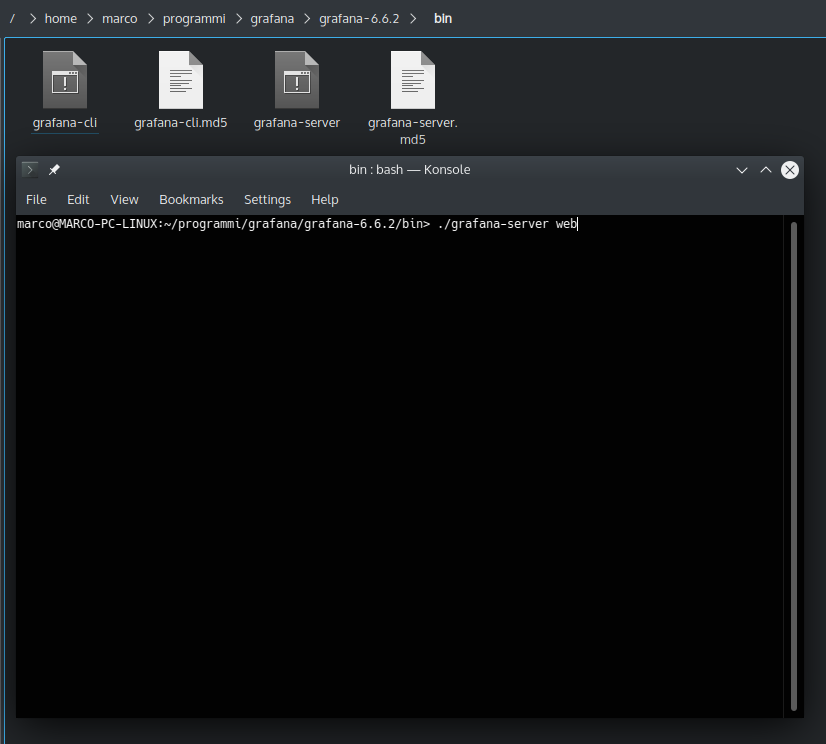
\includegraphics[width=10cm,height=\textheight,keepaspectratio]{img/grafana-server.png}
%\mbox{}\\ [5mm]
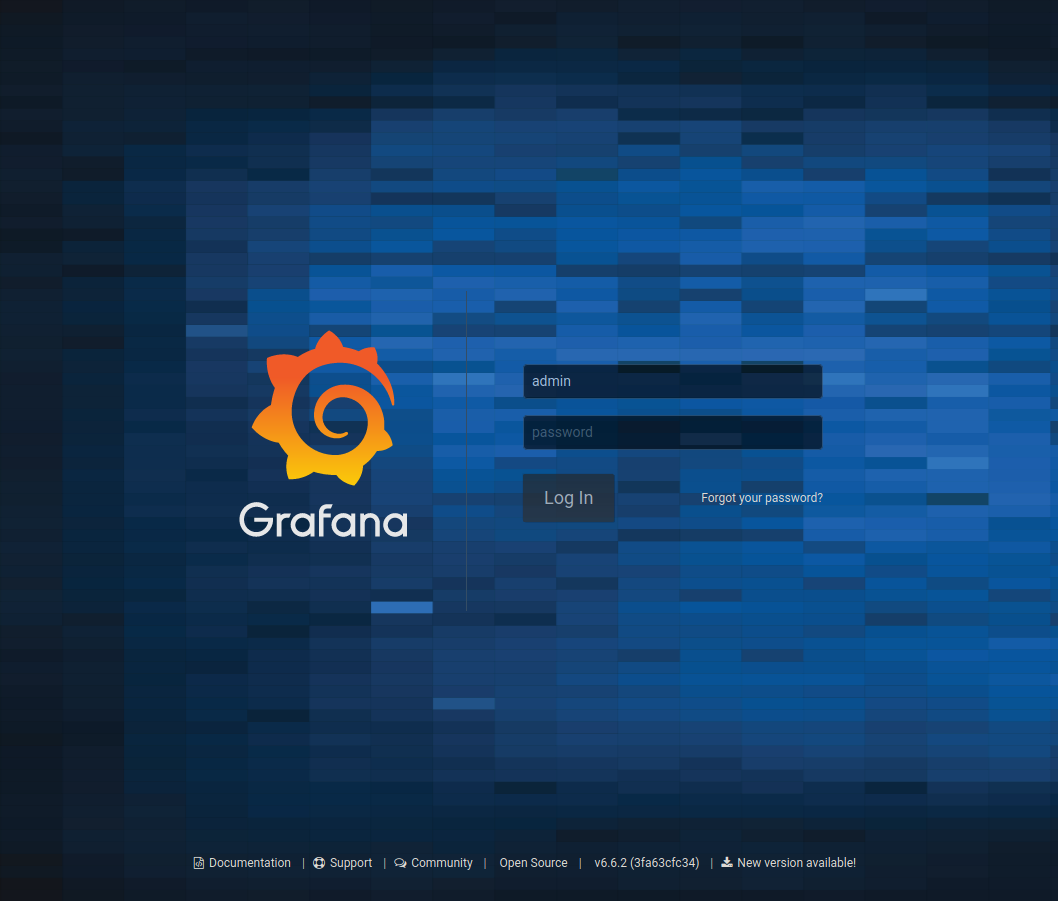
\includegraphics[width=10cm,height=\textheight,keepaspectratio]{img/grafana-login.png}
\end{center}

%\subsection{Installazione plug-in Grafana}
%\subsubsection{Requisiti}
%\begin{itemize}
%	\item \textbf{Grafana\glo};
%	\item \textbf{Node.js}: runtime Javascript che permette di eseguire codice Javascript fuori da un browser. L'installazione di npm (Node Package Manager) non è richiesta dato che viene installato automaticamente durante l'installazione di Node.js;
%	\item \textbf{Git}: sistema di versionamento distribuito.
%\end{itemize}

\subsection{Installazione del plug-in}
\subsubsection{Clonare la repository da GitHub}%\mbox{}\\ [1mm]
Per clonare la repository dell'applicazione, aprire un terminale e usare il comando cd per spostarsi in una cartella a propria scelta ed eseguire il comando:
\begin{verbatim}
	git clone https://github.com/VRAM-Software/grafana_prediction.git
\end{verbatim}
Infine con il comando 
\begin{verbatim}
	cd ./grafana_prediction_plugin
\end{verbatim}
si accede alla cartella che contiene il codice sorgente del plug-in.

\subsubsection{Installare le dipendenze}%\mbox{}\\ [1mm]
Per il corretto funzionamento dell'applicazione è necessario installare tutte le dipendenze elencate precedentemente. Per farlo eseguire il comando:
\begin{verbatim}
	npm install
\end{verbatim}

\subsubsection{Eseguire il plug-in}%\mbox{}\\ [1mm]
Per eseguire l'applicazione è necessario copiare il contenuto del repository "grafana\_prediction\_plugin", ad eccezione delle cartelle "node\_modules" e "coverage", all'interno della cartella "data/plugins" dell'installazione Grafana\glo. Accedendo all'interfaccia web si potrà quindi abilitare il plug-in dall'apposita sezione plug-in delle impostazioni.
\\
\\
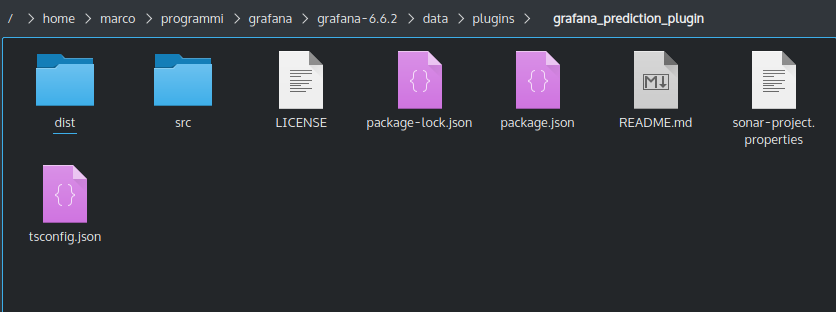
\includegraphics[width=\textwidth,height=\textheight,keepaspectratio]{img/plugin-directory.png}

\subsubsection{Impacchettare il plug-in}%\mbox{}\\ [1mm]
Per generare una release di produzione basta eseguire il comando:
\begin{verbatim}
	npm run build	
\end{verbatim}
e successivamente creare un archivio zip dell'intero repository escludendo le cartelle "node\_modules" e "coverage". Questo plug-in potrà poi esser distribuito e installato da altri utenti. 

	\subsection{Installazione dell'applicazione esterna a Grafana}
L'installazione dell'applicazione è suddivisa in due passaggi che descriviamo in dettaglio nei prossimi paragrafi:
\begin{enumerate}
    \item clonare la repository da GitHub;
    \item installare le dipendenze.
\end{enumerate}

\subsubsection{Clonare la repository da GitHub}%\mbox{}\\ [1mm]
Per clonare il repository dell'applicazione, aprire un terminale e usare il comando \texttt{cd} per spostarsi in una cartella a vostra scelta. Quindi per clonare il repository principale del nostro prodotto eseguire il comando:
\begin{verbatim}
	git clone https://github.com/VRAM-Software/grafana_prediction.git
\end{verbatim}
Infine per spostarsi nella cartella che contiene il codice sorgente dell'applicativo esterno si usa il comando:
\begin{verbatim}
	cd ./prediction_configuration_utility
\end{verbatim}

\begin{figure}[H] 	
	\begin{center}
		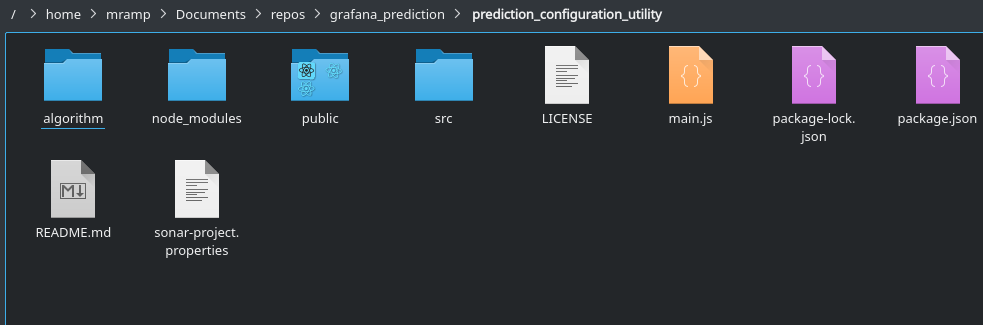
\includegraphics[width=\textwidth,height=\textheight,keepaspectratio]{img/directoryProject.png}
	\end{center}
	\caption{Selezione app nella directory}	
\end{figure}



\subsubsection{Installare le dipendenze}%\mbox{}\\ [1mm]
Per il corretto funzionamento dell'applicazione è necessario installare tutte le dipendenze elencate nel file \texttt{package.json}. Per farlo, eseguire da terminale nella cartella \verb|prediction_configuration_utility| il comando:
\begin{verbatim}
	npm install
\end{verbatim}
I pacchetti che vengono installati si suddividono in dipendenze e dipendenze sviluppatore.
%\\
%\\POCO VISIBILE
%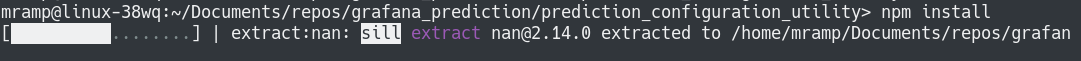
\includegraphics[width=\textwidth,height=\textheight,keepaspectratio]{img/packageInstallation.png}

\paragraph*{Dipendenze}\mbox{}\\ [1mm]
Nella seguente tabella sono elencate tutte le dipendenze necessarie per la corretta esecuzione dell'applicazione.
\mbox{}\\ [1mm]
\rowcolors{2}{gray!25}{gray!15}
	\setcounter{table}{0}
	\begin{longtable} {
		>{}p{65mm} 
		>{}p{30mm}
		}
    \rowcolor{gray!50}
    \textbf{Pacchetto} & \textbf{Versione} \TBstrut \\ [2mm]
    \verb|@testing-library/jest-dom| & \verb|^4.2.4|  \TBstrut \\ [2mm]
    \verb|@testing-library/react| & \verb|^9.3.2| \TBstrut \\ [2mm]
    \verb|@testing-library/user-event| & \verb|^7.1.2| \TBstrut \\ [2mm]
    \verb|csvtojson| & \verb|2.0.10| \TBstrut \\ [2mm]
    \verb|d3| & \verb|^5.15.0| \TBstrut \\ [2mm]
    \verb|electron-is-dev| & \verb|^1.1.0| \TBstrut \\ [2mm]
    \verb|ml-modules|\footnote{Il pacchetto \texttt{ml-modules} usato nel nostro progetto è una versione modificata dell'ononimo pacchetto} & \verb|0.1.0| \TBstrut \\ [2mm]
    \verb|precision-recall| & \verb|^1.0.2| \TBstrut \\ [2mm]
    \verb|react| & \verb|^16.13.0| \TBstrut \\ [2mm]
    \verb|react-dom| & \verb|^16.13.0| \TBstrut \\ [2mm]
    \verb|react-scripts| & \verb|3.4.0| \TBstrut \\ [2mm]
    \rowcolor{white}
    \caption{Dipendenze per eseguire applicazione}
    \end{longtable}
    
\paragraph*{Dipendenze sviluppatore}\mbox{}\\ [1mm]
Nella seguente tabella sono elencate tutte le dipendenze necessarie per la corretta esecuzione dell'applicazione durante lo sviluppo.
\rowcolors{2}{gray!25}{gray!15}
	\setcounter{table}{1}
	\begin{longtable} {
		>{}p{65mm} 
		>{}p{30mm}
		}
    \rowcolor{gray!50}
    \textbf{Pacchetto} & \textbf{Versione} \TBstrut \\ [2mm]
    \verb|electron| & \verb|^8.02| \TBstrut \\ [2mm]
    \verb|electron-packager| & \verb|^14.2.1| \TBstrut \\ [2mm] 
    \verb|coveralls| & \verb|^3.0.9| \TBstrut \\ [2mm]
    \verb|enzyme| & \verb|^3.11.0| \TBstrut \\ [2mm]
    \verb|enzyme-adapter-react-16| & \verb|^1.15.2| \TBstrut \\ [2mm]
    \verb|prettier| & \verb|^2.0.5| \TBstrut \\ [2mm]
    \verb|spectron| & \verb|^10.0.1| \TBstrut \\ [2mm]
    \rowcolor{white}
    \caption{Dipendenze specifiche per lo sviluppatore}
    \end{longtable}
    \mbox{}\\ [1mm]
Seguendo i due passaggi descritti nei precedenti paragrafi, l'applicazione esterna è installata correttamente.

\subsubsection{Eseguire l'applicazione}%\mbox{}\\ [1mm]
Per eseguire il l'applicazione è necessario aprire due terminali nella cartella: "prediction\_configuration\_utility", eseguire nel primo il comando \verb|npm start| per inizializzare il server Node.Js alla porta 3000. Infine, nel secondo terminale, eseguire il comando \verb|npm run electron| per inizializzare l'istanza di Electron.

\subsubsection{Impacchettare l'applicazione}%\mbox{}\\ [1mm]
Per generare una release di produzione eseguire il seguente comando per:
\begin{verbatim}
  npm run build 
\end{verbatim}
In seguito, a seconda del sistema operativo utilizzato, eseguire uno dei seguenti comandi:
\begin{verbatim}
  npm run package-win
  npm run package-mac
  npm run package-linux
\end{verbatim}

\pagebreak
\subsection{Installazione ambiente di sviluppo integrato WebStorm}
Per installare l'ambiente di sviluppo integrato WebStorm, visitare la pagina \url{https://www.jetbrains.com/webstorm/download/}. Qui è possibile trovare il download per MacOS, Windows e sistemi operativi basati su Linux/Unix.
\\
%\\
%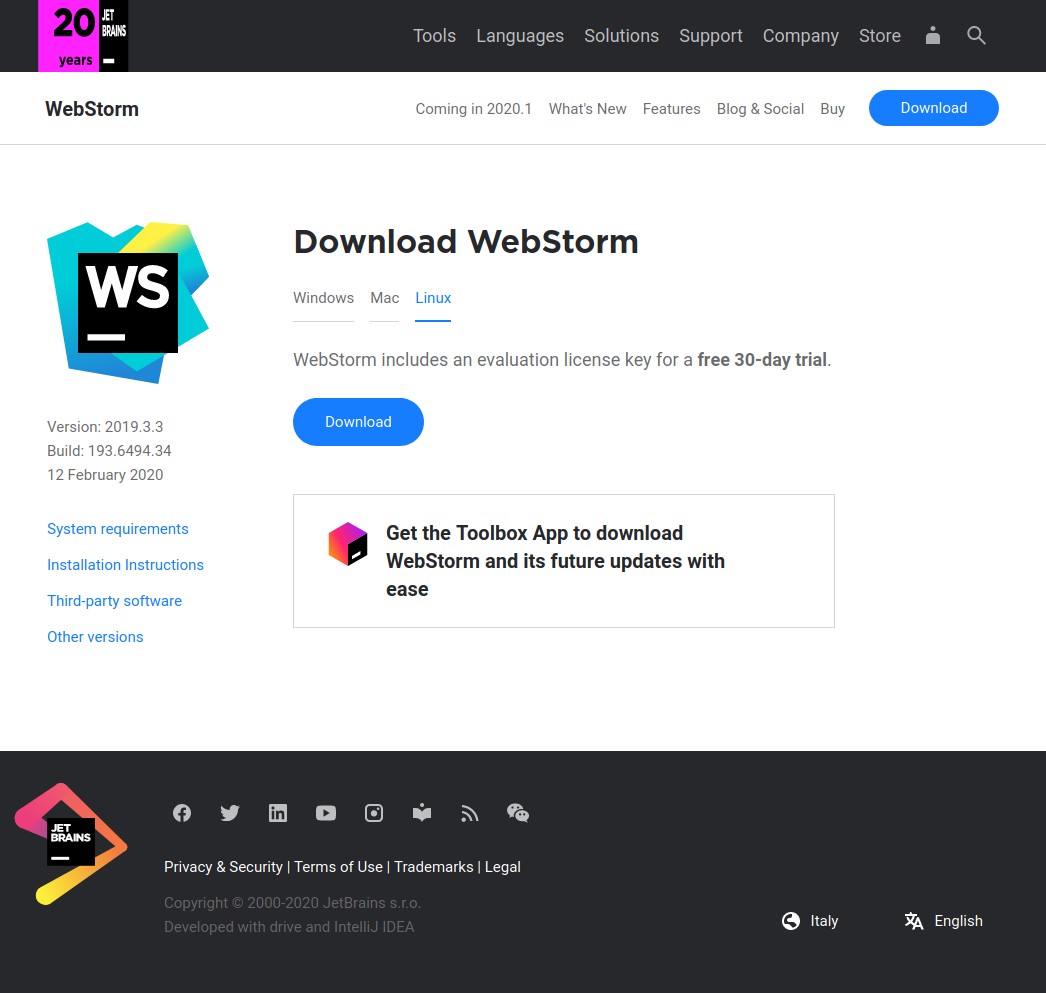
\includegraphics[width=\textwidth,height=\textheight,keepaspectratio]{img/webstorm.png}

%\pagebreak
\subsubsection{Installazione plug-in SonarLint per WebStorm}
Per installare il plug-in SonarLint per WebStorm, aprire le impostazioni di WebStorm dal suo menù "File". Quindi nella sezione "Plugins" cercare ed installare "SonarLint".
\\
\\
\begin{figure}[H] 	
	\begin{center}
		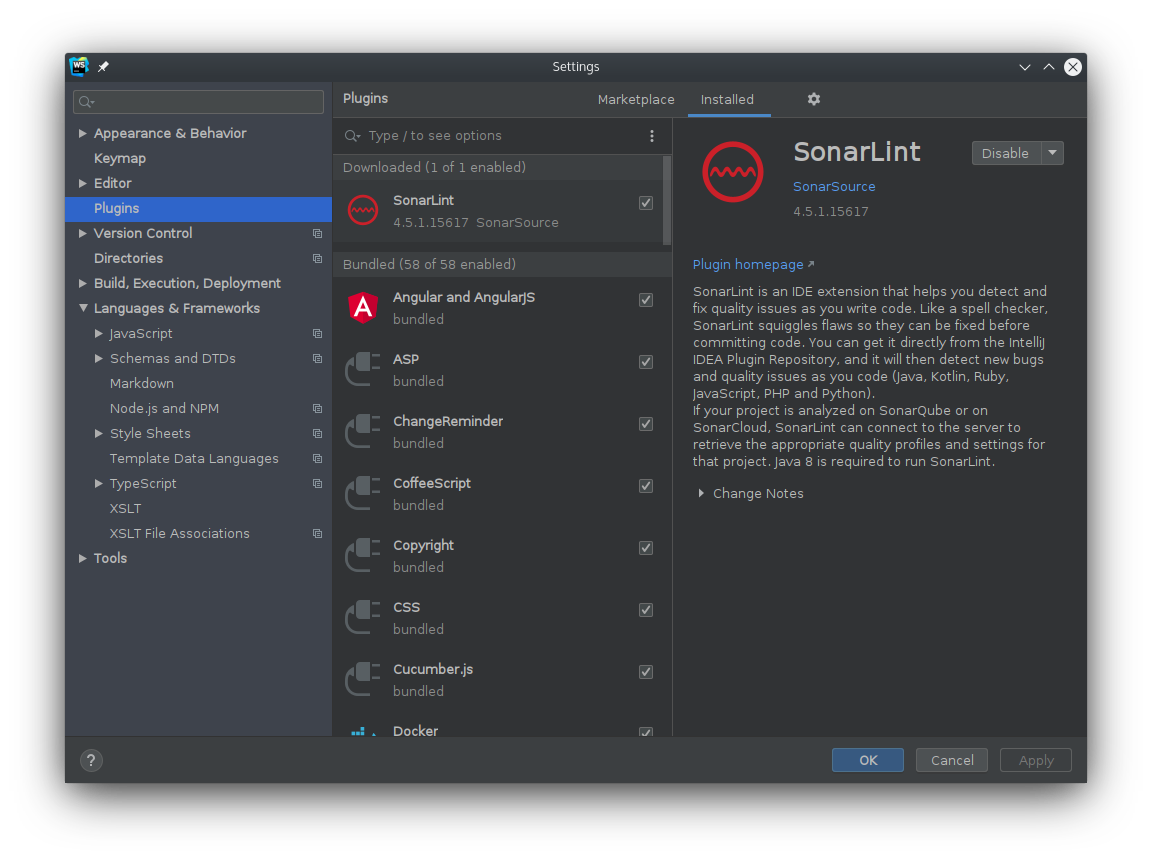
\includegraphics[width=\textwidth,height=\textheight,keepaspectratio]{img/sonarlint.png}
	\end{center}
	\caption{Installazione SonarLint}	
\end{figure}


	\pagebreak
	\section{Configurazione dell'ambiente di lavoro}
\subsection{Configurazione ambiente di sviluppo integrato WebStorm}
La configurazione base di WebStorm prevede la corretta configurazione dei path di sistema e l'apertura di un progetto.
\subsubsection{Configurazione dei path di sistema}
Aprire le impostazioni di WebStorm dal suo menù "File" ed utilizzando la barra di ricerca cercare "Node.js and NPM". Verificare quindi che entrambe le voci "Node interpreter" e "Package manager" siano correttamente impostate.
\\
\\
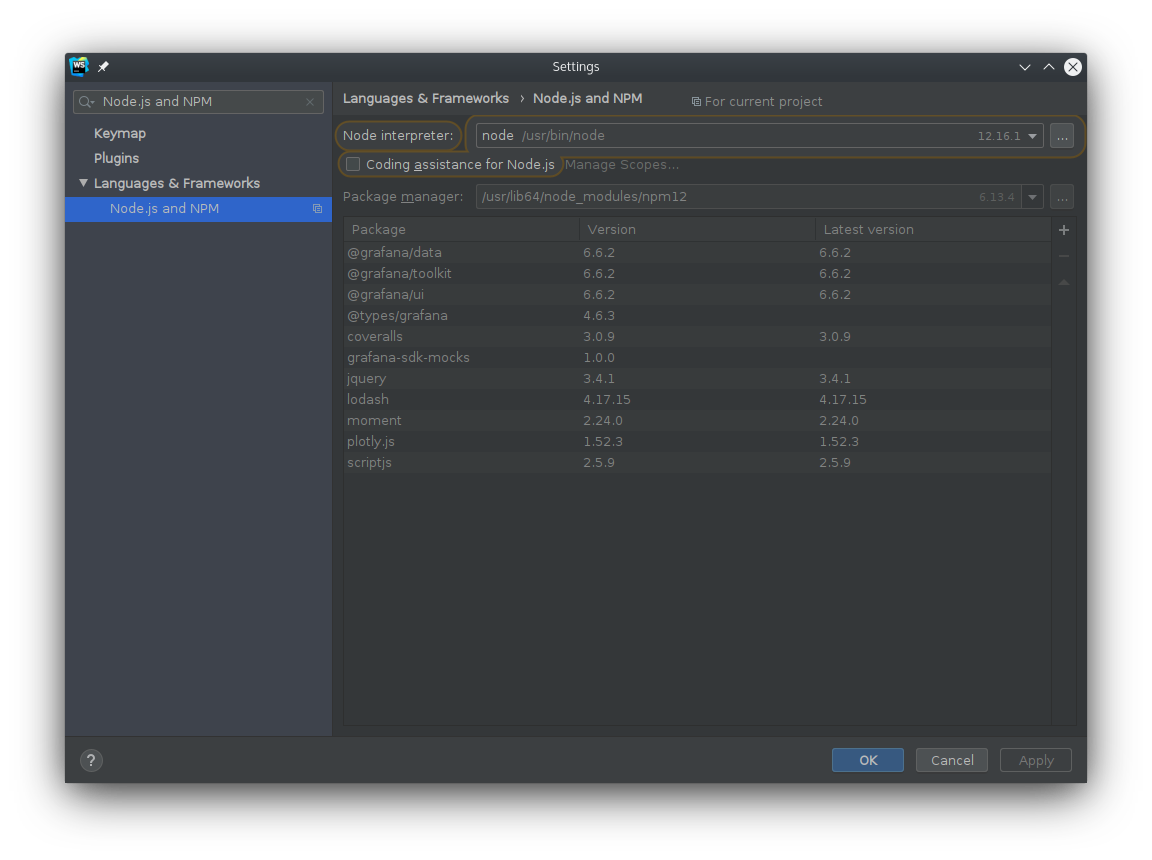
\includegraphics[width=\textwidth,height=\textheight,keepaspectratio]{img/node-npm.png}
\subsubsection{Importazione di un progetto}
Dal menu "File" selezionare la voce "Open" e successivamente la root directory del repository desiderato.

\pagebreak
\subsection{Configurazione plug-in SonarLint per WebStorm}
\subsubsection{Configurazione globale}
Per configurare il plug-in SonarLint, aprire le impostazioni di WebStorm dal suo menù "File". Quindi nella sezione "Tools" selezionare la voce "SonarLint". Nella finestra visualizzare selezionare il "+" per aggiungere una connessione al servizio WEB SonarCloud.
\\
\\
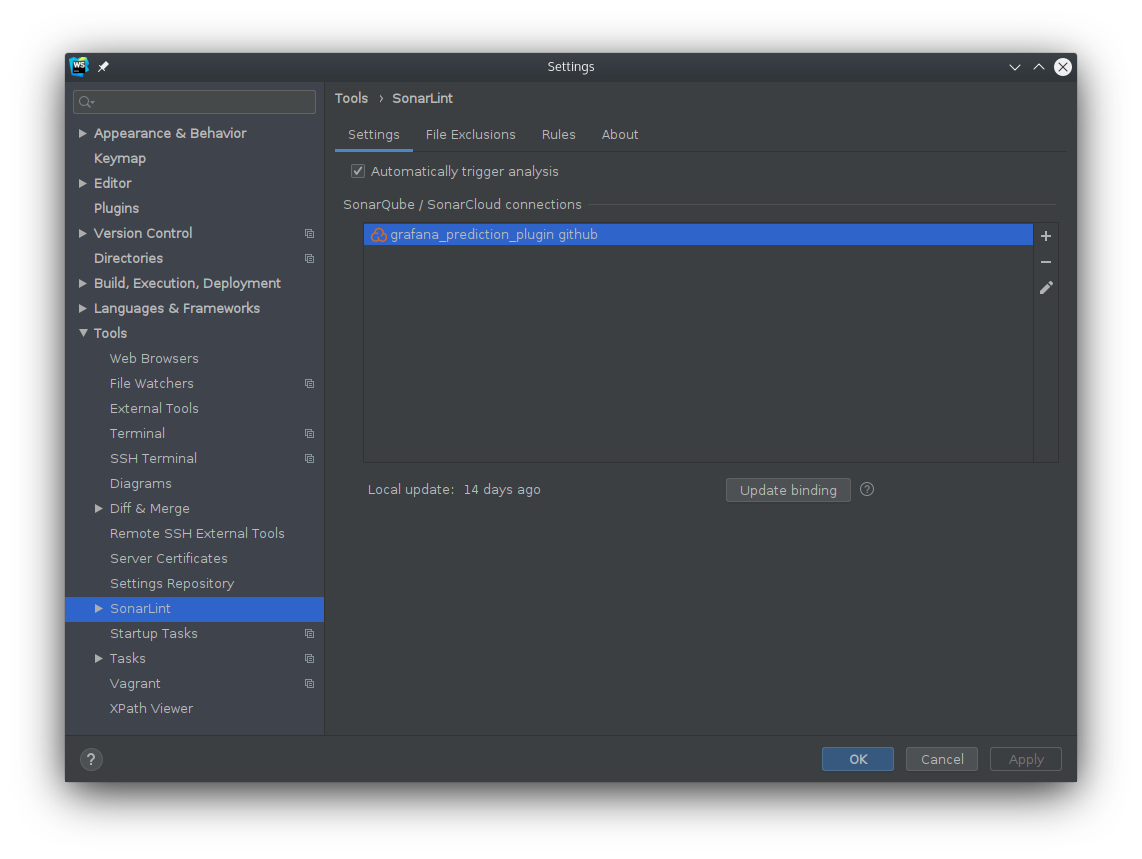
\includegraphics[width=\textwidth,height=\textheight,keepaspectratio]{img/connection.png}
\pagebreak
\\
Dare un nome al collegamento e selezionare SonarCloud, successivamente premere "Next".
\\
\\
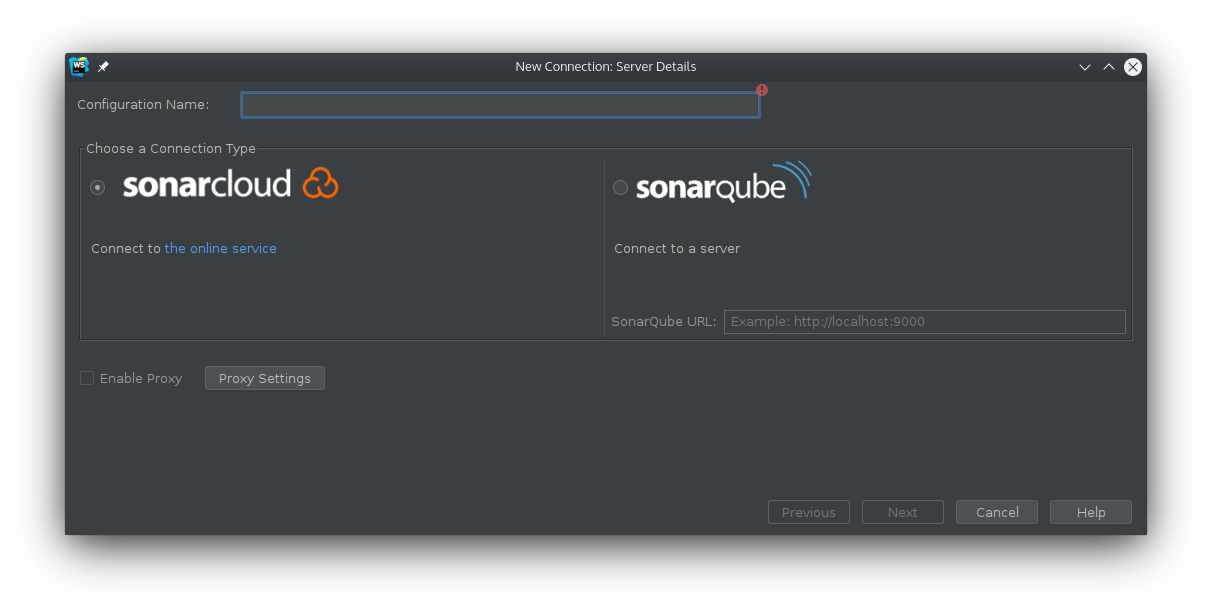
\includegraphics[width=\textwidth,height=\textheight,keepaspectratio]{img/connection-name.png}
\\
Premere su "Create Token".
\\
\\
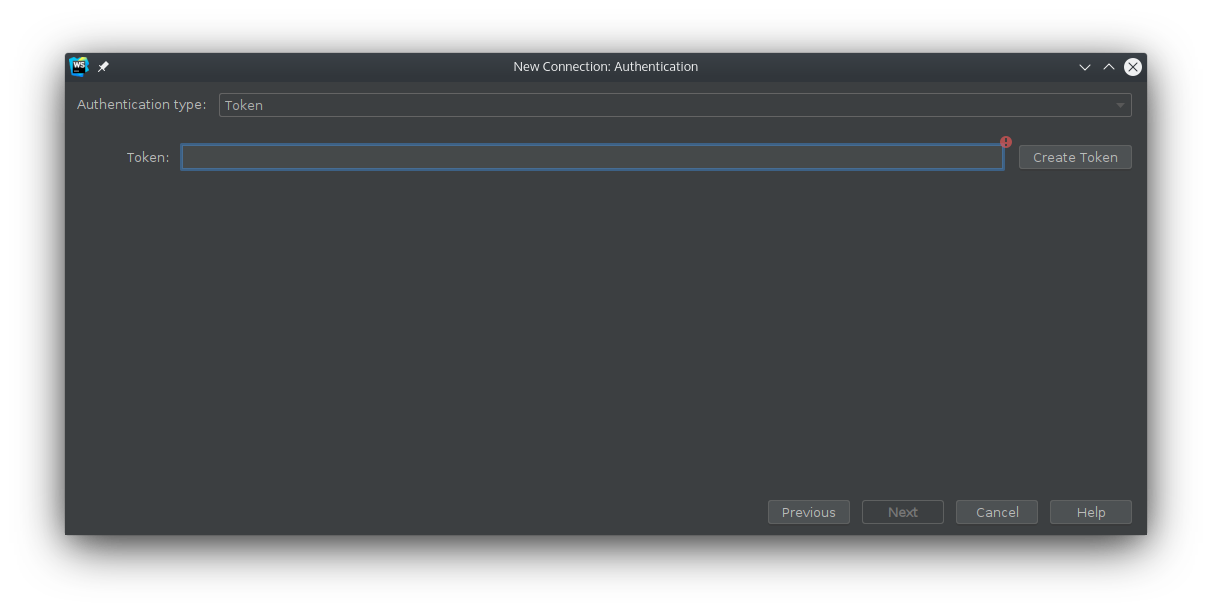
\includegraphics[width=\textwidth,height=\textheight,keepaspectratio]{img/token.png}
\\
Scegliere un nome e creare il token, copiarlo quindi nella finestra WebStorm precedente.
%\\
%\\
%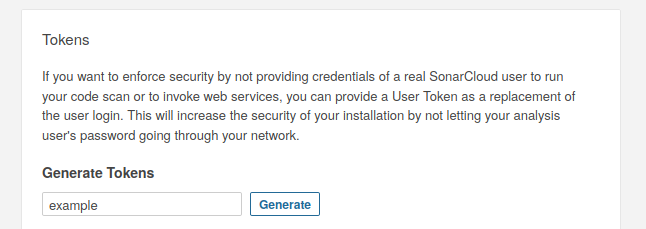
\includegraphics[width=\textwidth,height=\textheight,keepaspectratio]{img/sonarcloud.png}
La connessione viene verificata ed è possibile visualizzarla nell'elenco delle connessioni.
\subsubsection{Configurazione per progetto}
Dopo aver terminato la configurazione globale è possibile configurare i singoli progetti. Per farlo aprire le impostazioni di WebStorm dal suo menù "File", Quindi nella sezione "Tools" espandere la voce "SonarLint" e selezionare "Project Settings".
\\
\\
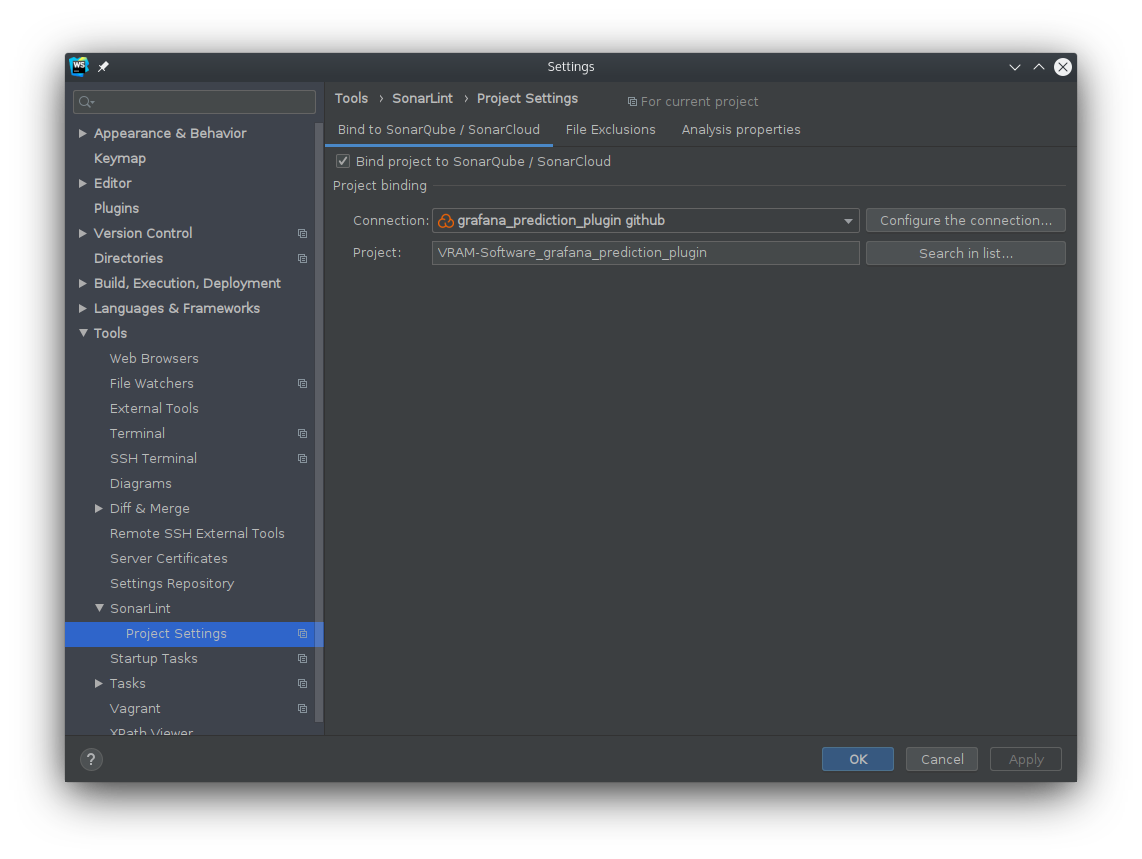
\includegraphics[width=\textwidth,height=\textheight,keepaspectratio]{img/sonarlint-project.png}
Selezionare la connessione a SonarCloud desiderata ed inserire una delle chiavi seguenti, a seconda del progetto che si sta configurando:
\begin{itemize}
	\item \textbf{plug-in Grafana}: VRAM-Software\_grafana\_prediction\_plugin;
	\item \textbf{Applicativo esterno}: VRAM-Software\_prediction\_configuration\_utility.
\end{itemize}

\subsection{Configurazione ambiente plug-in Grafana}
\subsubsection{Contenuto file package.json}
Il file package.json contiene tutte le informazioni e i requisiti necessari della nostra applicazione. Le informazioni importanti sono i seguenti attributi:
\begin{itemize}
	\item dependencies: contiene la seguente lista di pacchetti che sono necessari per il corretto funzionamento dell'applicazione:
		\begin{itemize}
			\item jquery;
			\item lodash;
			\item moment;
			\item plotly.js;
			\item scriptjs.
		\end{itemize}
	\item devDependencies: questo attributo contiene la seguente lista di pacchetti che sono necessari per il corretto funzionamento dell'applicazione durante lo sviluppo:
		\begin{itemize}
			\item @grafana/data;
			\item @grafana/toolkit;
			\item @grafana/ui;
			\item @types/grafana;
			\item grafana-sdk-mocks;
			\item coveralls.
		\end{itemize}
	\item{scripts}: questo attributo contiene una lista di tutti i comandi, utili per uno sviluppatore, che possono essere eseguiti da linea di comando:
		\begin{itemize}
			\item \textbf{build}: il comando seguente genera una cartella chiamata dist che contiene i file di produzione del plug-in Grafana\glo;
			\begin{verbatim}
				npm run build
			\end{verbatim}
			\item \textbf{test}: il comando fa eseguire tutti i test automatici dell'applicazione;
			\begin{verbatim}
				npm test
			\end{verbatim}
			\item \textbf{dev}: il comando genera una release di debug da utilizzare durante lo sviluppo, eseguendo inoltre i linting integrati nella dipendenza npm @grafana/toolkit. Non esegue i test automatici;
			\begin{verbatim}
				npm run dev
			\end{verbatim}
			\item \textbf{ci-test}: il comando, pensato per essere eseguito nell'ambiente di continuous integration, fa eseguire tutti i test automatici dell'applicazione e calcola il code coverage del codice;
			\begin{verbatim}
				npm run ci-test
			\end{verbatim}
			\item \textbf{watch}: il comando esegue il comando "dev" in modalità "watch", ovvero segnalando in automatico gli errori di linting durante la scrittura del codice.
			\begin{verbatim}
				npm run watch
			\end{verbatim}
		\end{itemize}
\end{itemize}

	\subsection{Configurazione ambiente applicativo esterno}
\subsubsection{Contenuto file: package.json}
Il file \verb|package.json | contiene tutte le informazioni e le dipendenze necessarie della nostra applicazione.
\begin{itemize}
    \item \textbf{"main"}: questo elemento ha come valore il percorso del file che si occupa di gestire il processo principale dell'applicazione Electron;
    \item \textbf{"dependencies"}: questo elemento contiene la seguente lista di pacchetti che sono necessari per il corretto funzionamento dell'applicazione:
        \begin{itemize}
            \item csvtojson;
            \item d3;
            \item electron-is-dev;
            \item ml-modules;
            \item precision-recall;
            \item react;
            \item react-dom;
            \item react-router-dom;
            \item react-scripts.
        \end{itemize}
    \item \textbf{"devDependencies"}: questo elemento contiene la seguente lista di pacchetti necessari per il corretto funzionamento dell'applicazione durante lo sviluppo:
        \begin{itemize}
            \item electron;
            \item electron-packager;
            \item coveralls;
            \item prettier;
            \item enzyme;
            \item enzyme-adapter-react-16;
            \item spectron.
        \end{itemize} 
    \item \textbf{"scripts"}: questo elemento contiene una lista di tutti i comandi, utili per uno sviluppatore, che possono essere eseguiti da linea di comando:
        \begin{itemize}
            \item \textbf{electron}: il comando seguente avvia un'istanza di Electron;
            \begin{verbatim}
            	npm run electron
            \end{verbatim}
            \item \textbf{start}: il comando seguente avvia un server Node.js alla porta 3000;
            \begin{verbatim}
	            npm start
            \end{verbatim}
            \item \textbf{build}: il comando seguente genera una cartella: \verb|build| che contiene i file di produzione di React;
            \begin{verbatim}
            	npm build
            \end{verbatim}
            \item \textbf{test}: il comando seguente esegue tutti i test dell'applicazione;\\
            \begin{verbatim}
            	npm test
            \end{verbatim}
            \item \textbf{beautify}: il comando seguente esegue un controllo e correzione dell'indentazione del codice;\\
            \begin{verbatim}
            	npm run beautify
            \end{verbatim}
            \item \textbf{package-mac}: il comando seguente genera una release di produzione\glosp per il sistema operativo: MacOS;
            \begin{verbatim}
            	npm run package-mac
            \end{verbatim}
            \item \textbf{package-win}: il comando seguente genera una release di produzione\glosp per il sistema operativo: Windows;
            \begin{verbatim}
            	npm run package-win
            \end{verbatim}
            \item \textbf{package-linux}: il comando seguente genera una release di produzione\glosp per una qualsiasi distribuzione di Linux.
            \begin{verbatim}
            	npm run package-linux
            \end{verbatim}
        \end{itemize}
\end{itemize}

	\pagebreak
	\section{Test}
	\subsection{Applicativo di addestramento}
		\subsubsection{Esecuzione dei test}
			Una volta avviato il server NodeJS, i test di unità si avvieranno con il comando \textbf{npm test} e scegliere l'opzione \textbf{a}, che avvierà i test con Enzyme e Jest. I risultati dei test verranno visualizzati direttamente nel terminale, inoltre i test verranno rieseguiti automaticamente alla modifica del codice.
		\subsubsection{Scrittura dei test}
			Per ogni componente viene creato un file di test, con il nome \textbf{<nome componente>.test.js}, all'interno del quale verranno definiti i test con Enzyme. Vengono verificati sia il corretto caricamento dei componenti che la correttezza del loro comportamento, assegnando uno stato e verificando i risultati in seguito alle chiamate dei metodi.
	\subsection{SonarCloud}
		SonarCloud misura la qualità del codice, ad ogni commit infatti analizza i sorgenti ed estrae indici su manutenibilità, complessità, affidabilità, duplicazione del codice, numero di bug e vulnerabilità... L'obiettivo è quello di avere codice sempre in buono stato e pronto al rilascio.
	\subsection{Coperatura dei test}
		La copertura dei test viene misurata da Coveralls, che ad ogni nuovo commit verifica la copertura dei test e ne mantiene uno storico. Per accedere alle statistiche sulla copertura dei test, premere sull'apposito badge nelle repository\glo, che aprirà la rispettiva pagina sul sito di Coveralls.

	\pagebreak
	\section{Tecnologie utilizzate}
	\subsection{Electron}
		Electron è un framework che permette di sviluppare applicazioni desktop utilizzando tecnologie web, basandosi sul motore di rendering di chromium. Viene utilizzato dall'applicativo di addestramento come contenitore dell'app
	\subsection{React}
		React è un framework JavaScript che si occupa prevalentemente della gestione dell'interfaccia, permettendo di dividerla in componenti modulari e riutilizzabili.
	\subsection{AngularJS}
		AngularJS è un framework JavaScript che si basa su un pattern MVC/MVVM per la realizzazione di applicazioni web. È l'alternativa più popolare per lo sviluppo di plug-in per Grafana\glo.
	\subsection{NodeJS}
		NodeJS è una runtime JavaScript, ovvero un ambiente di esecuzione per codice JavaScript; viene impiegato nella fase di sviluppo come server web per l'applicazione esterna.
	\subsection{JSX}
		JSX è un'estensione del linguaggio JavaScript che viene utilizzata per definire la struttura e la logica dei componenti in React, presenta una sintassi simile al linguaggio HTML.
	\subsection{Jest}
		Jest è un framework per i test di unità dei componenti JavaScript, viene utilizzato con Enzyme per i test dell'applicativo di addestramento.
	\subsection{Enzyme}
		Enzyme è uno strumento di test JavaScript specifico per componenti React, si integra con Jest.
	\subsection{SonarLint}
		SonarLint è un plug-in per IDE che attraverso l'analisi statica\glosp del codice rileva anomalie ed errori comuni. Provvede quindi a segnalare queste vulnerabilità e proporre eventuali soluzioni.
	\subsection{NPM}
		Il Node Package Manager viene utilizzato per la gestione delle dipendenze e la build automation.
		Richiede che all'interno del progetto sia presente il file package.json, che contiene informazioni riguardanti le dipendenze e gli script di build e test.
	\subsection{D3}
		D3 è una libreria JavaScript per produrre visualizzazioni di dati dinamiche e interattive. Impiegata per creare i grafici nell'applicativo di addestramento.
	\subsection{Plotly}
		Plotly è un'altra libreria JavaScript per la visualizzazione di dati, si basa su D3, viene utilizzata dal plug-in per produrre grafici in Grafana\glo.
	\subsection{TypeScript}
		TypeScript è un'estensione del linguaggio JavaScript che aggiunge il supporto ai tipi, viene usato nei plug-in di Grafana\glo.
	\subsection{JSON}
		JSON è un formato per lo scambio di dati derivato da JavaScript, viene utilizzato per memorizzare risultati e informazioni degli addestramenti.
	\subsection{CSV}
		CSV è un formato per lo scambio di dati, viene usato per la memorizzazione dei dati di test.
	\subsection{InfluxDB}
		InfluxDB è un time series database, cioè una base di dati che memorizza le informazioni come coppie di valori tempo e dato. Proprio per questo motivo è una delle fonti di dati predilette da Grafana\glo.
	\subsection{Regressione lineare}
		La regressione lineare è un modello di regressione che, a partire da un insieme di dati rappresentabili come punti su un piano, restituisce una stima sul loro sviluppo sotto forma di retta.
	\subsection{Support-vector machines}
		Le support-vector machines sono modelli di apprendimento supervisionati che vengono utilizzati nell'ambito del machine learning\glo: a partire da una serie di dati questi vengono analizzati e viene effettuata una classificazione che li divide in due sottoinsiemi.




	\pagebreak
	%ARCHITETTURA PLUG-IN
\section{Architettura del prodotto}
Il nostro prodotto\glosp è composto da un plug-in sviluppato per la piattaforma Grafana\glosp e un'applicazione ausiliaria, esterna a tale piattaforma. Perciò l'analisi dell'architettura è suddivisa in queste due componenti.
\subsection{Plug-in}
Per poter visualizzare la suddivisione delle componenti del plug-in e le dipendenze che sussistono tra loro ad alto livello, viene riportato il diagramma dei Package in allegato nel file \textit{diagramma-package-plug-in.png}.
\subsubsection{Progettazione architetturale}
Abbiamo deciso di utilizzare un design pattern architetturale Model-View-Controller (MVC) perché si adatta bene allo sviluppo software all'interno di Grafana\glo. In particolare, come si può vedere nella figura seguente, abbiamo la View che scambia informazioni sulle interazioni dell'utente con il Controller che a sua volta le trasforma in azioni sui dati eseguite da Model. Infine vi è una comunicazione tra Model e View per il costante aggiornamento di quest'ultima, grazie ad una funzionalità fornita dalla piattaforma Grafana\glo.
\mbox{}
\begin{landscape}
	\begin{figure}
		\begin{figure} [H]
			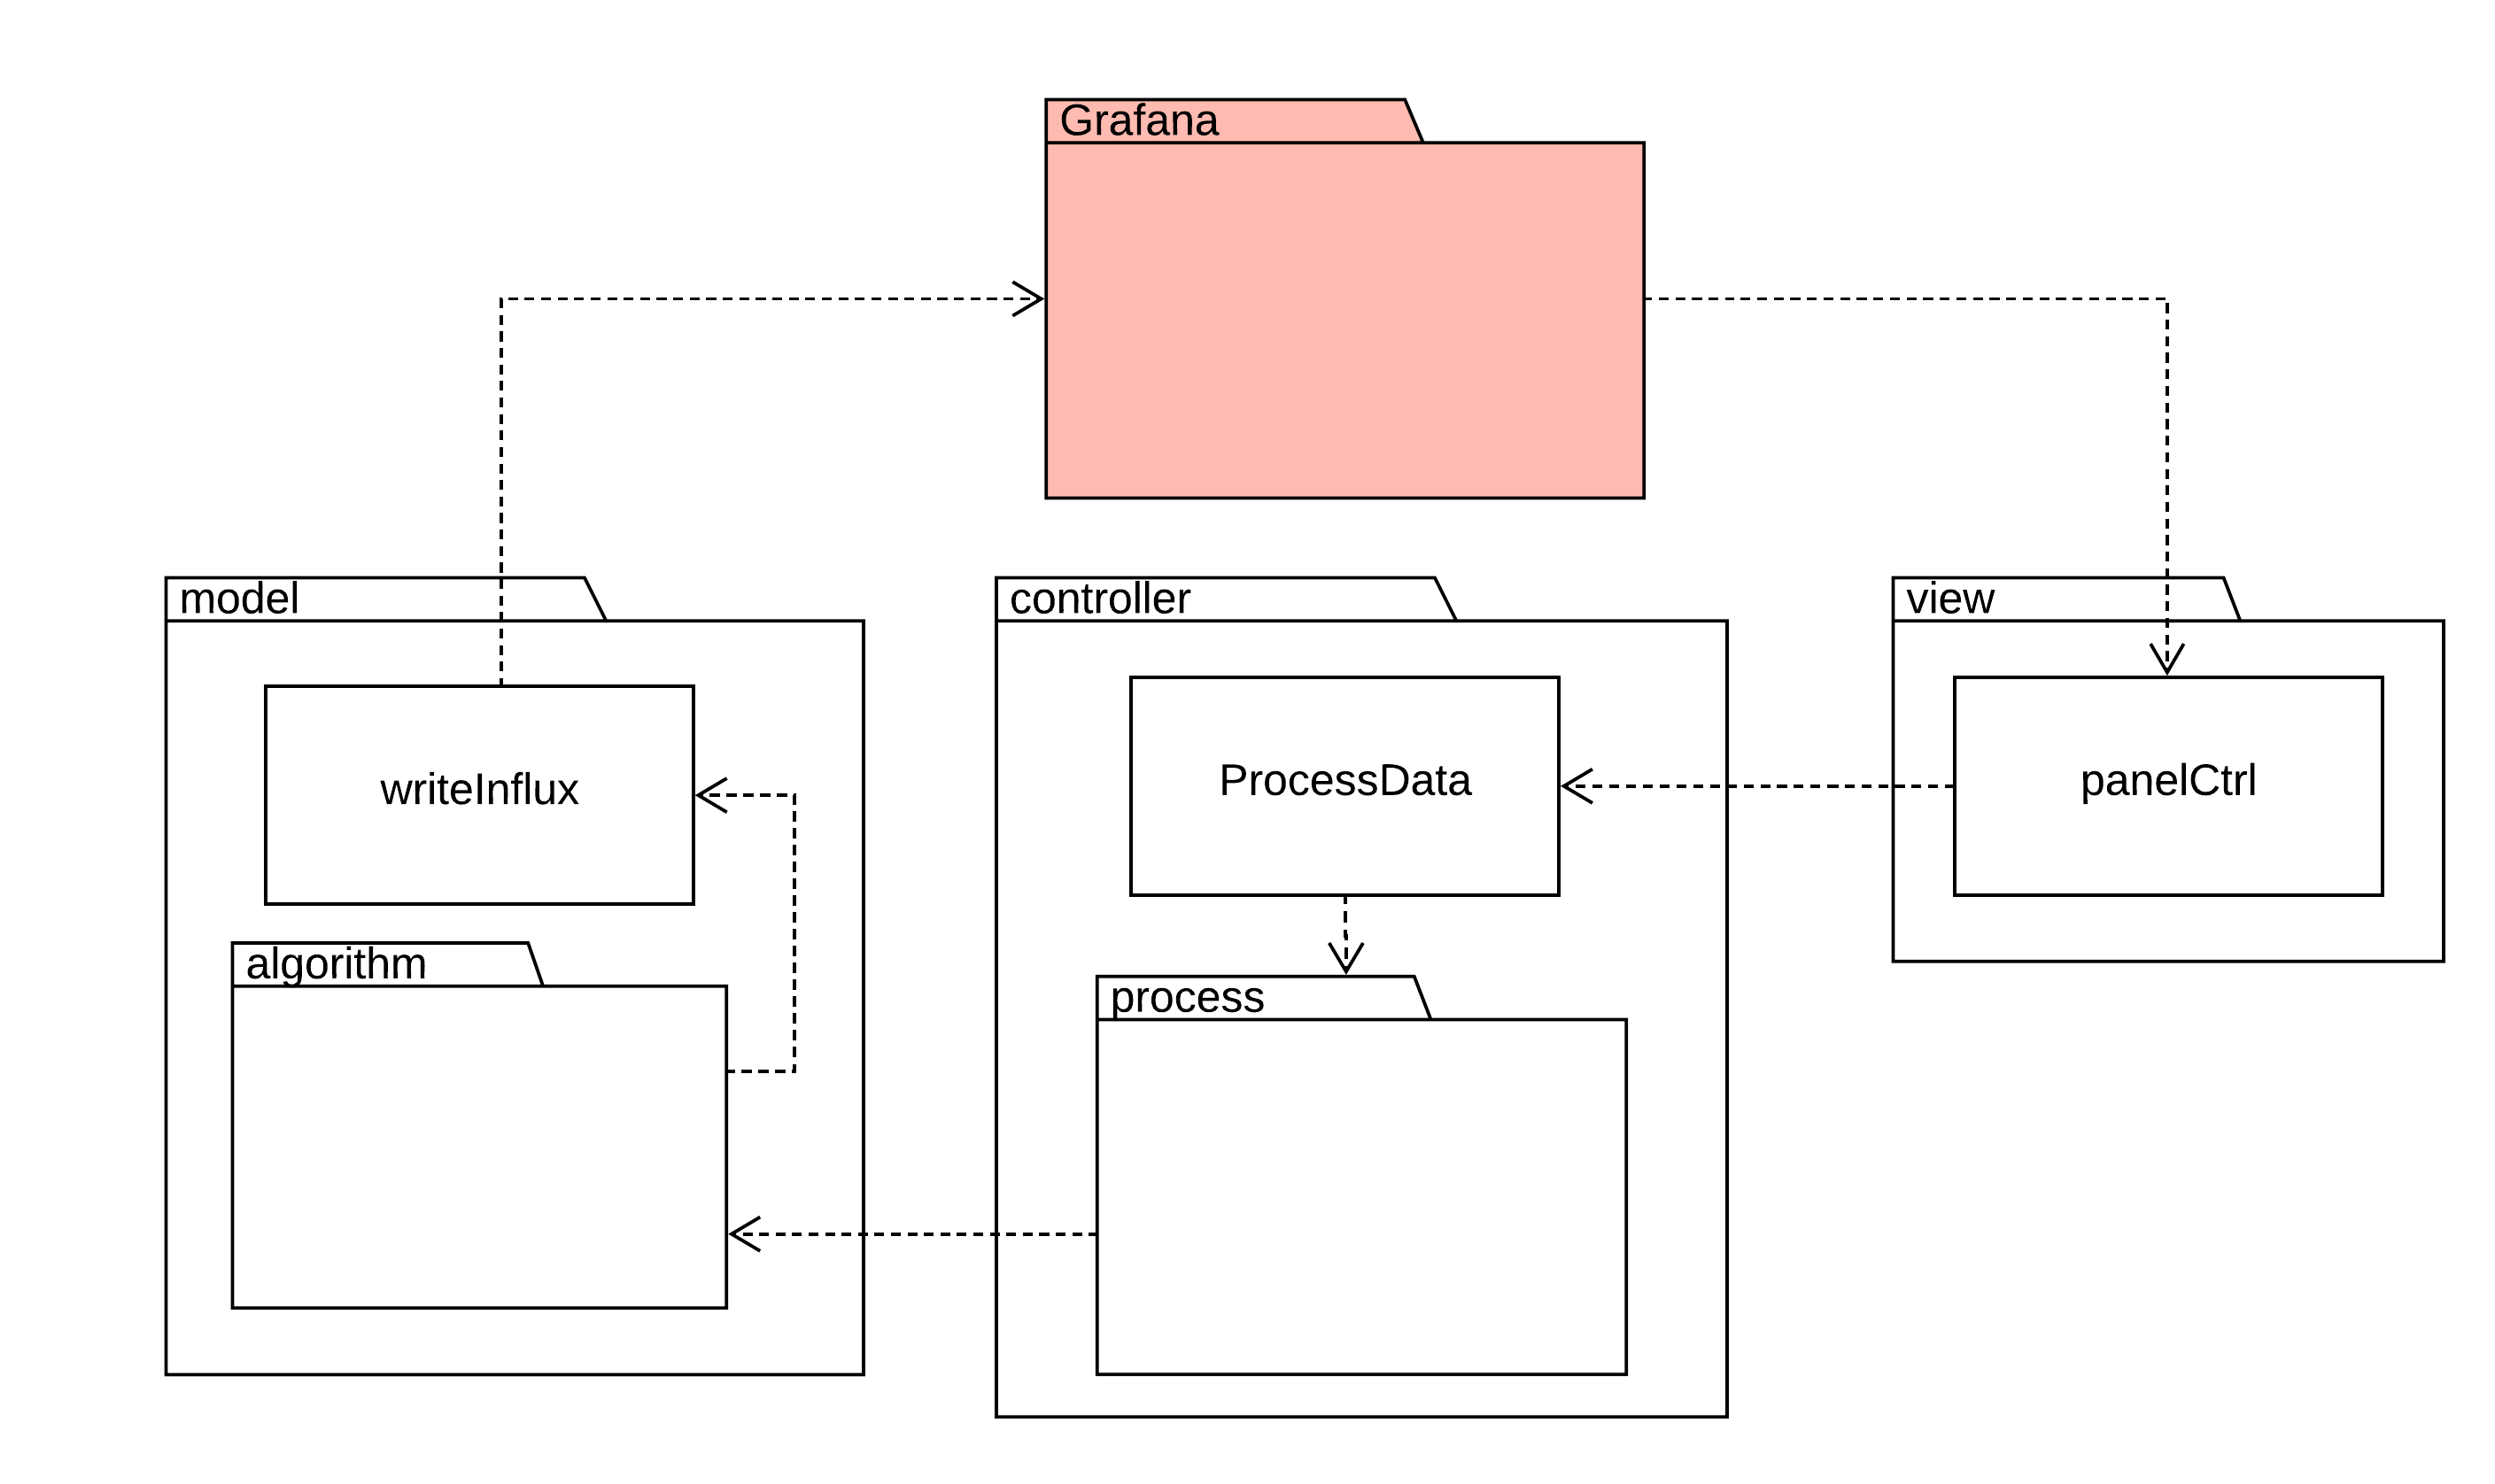
\includegraphics[width=\linewidth]{./img/Diagrammi/architettura-plug-in.png}
			\caption{Diagramma dell'architettura del plug-in}
		\end{figure}
	\end{figure}
\end{landscape}
Analizzando i componenti, la nostra architettura è così strutturata: 
\begin{itemize}
	\item \textbf{Model}: modulo che gestisce la business logic. Più in dettaglio contiene gli algoritmi di predizione dei dati che sono stati implementati, la lettura dei dati di input ed infine la scrittura del risultato delle predizioni su un database Influx;
	\item \textbf{View}: modulo che gestisce la presentation logic. Più in dettaglio permette la creazione di una pannello personalizzato della dashboard di Grafana\glosp dal quale l'utente può interagire;
	\item \textbf{Controller}: modulo che gestisce l'application logic. Più in dettaglio vengono trasformate le interazioni dell'utente in un formato adatto per l'esecuzione corrispettiva delle azioni da parte del Model.
\end{itemize}
\subsubsection{Progettazione di dettaglio}
Di seguito viene descritta in dettaglio la progettazione del plug-in. In allegato viene fornito il file \textit{diagramma-classi-plug-in.png} contenente l'intero diagramma delle classi.
\paragraph{Model} \mbox{}
L'elemento principale contenuto all'interno del modello è il componente degli algoritmi di predizione. Abbiamo implementato due algoritmi di predizione: Support Vector Machine lineare\glosp e Regressione lineare\glo. Esse sono rappresentate rispettivamente dalle classi concrete \textit{SvmPrediction} e \textit{RlPrediction}. In senso più generale abbiamo riscontrato che per le famiglie di algoritmi di Support Vector Machine e di Regressione è possibile ricondursi ad un'interfaccia unica che abbiamo chiamato \textit{AlgorithmPrediction}. Essa fornisce il metodo astratto \textit{predict(data, configuration, influxParameter)} che è implementato dalle classi concrete dei singoli algoritmi.
Queste due classi hanno una dipendenza di tipo composizione con la classe concreta \textit{WriteInflux} che importa la libreria \textit{InfluxDB} e contiene le funzionalità di scrittura su un database Influx. Essa presenta due metodi per la scrittura sul database.
\mbox{}
\begin{landscape}
	\begin{figure}
		\begin{figure} [H]
			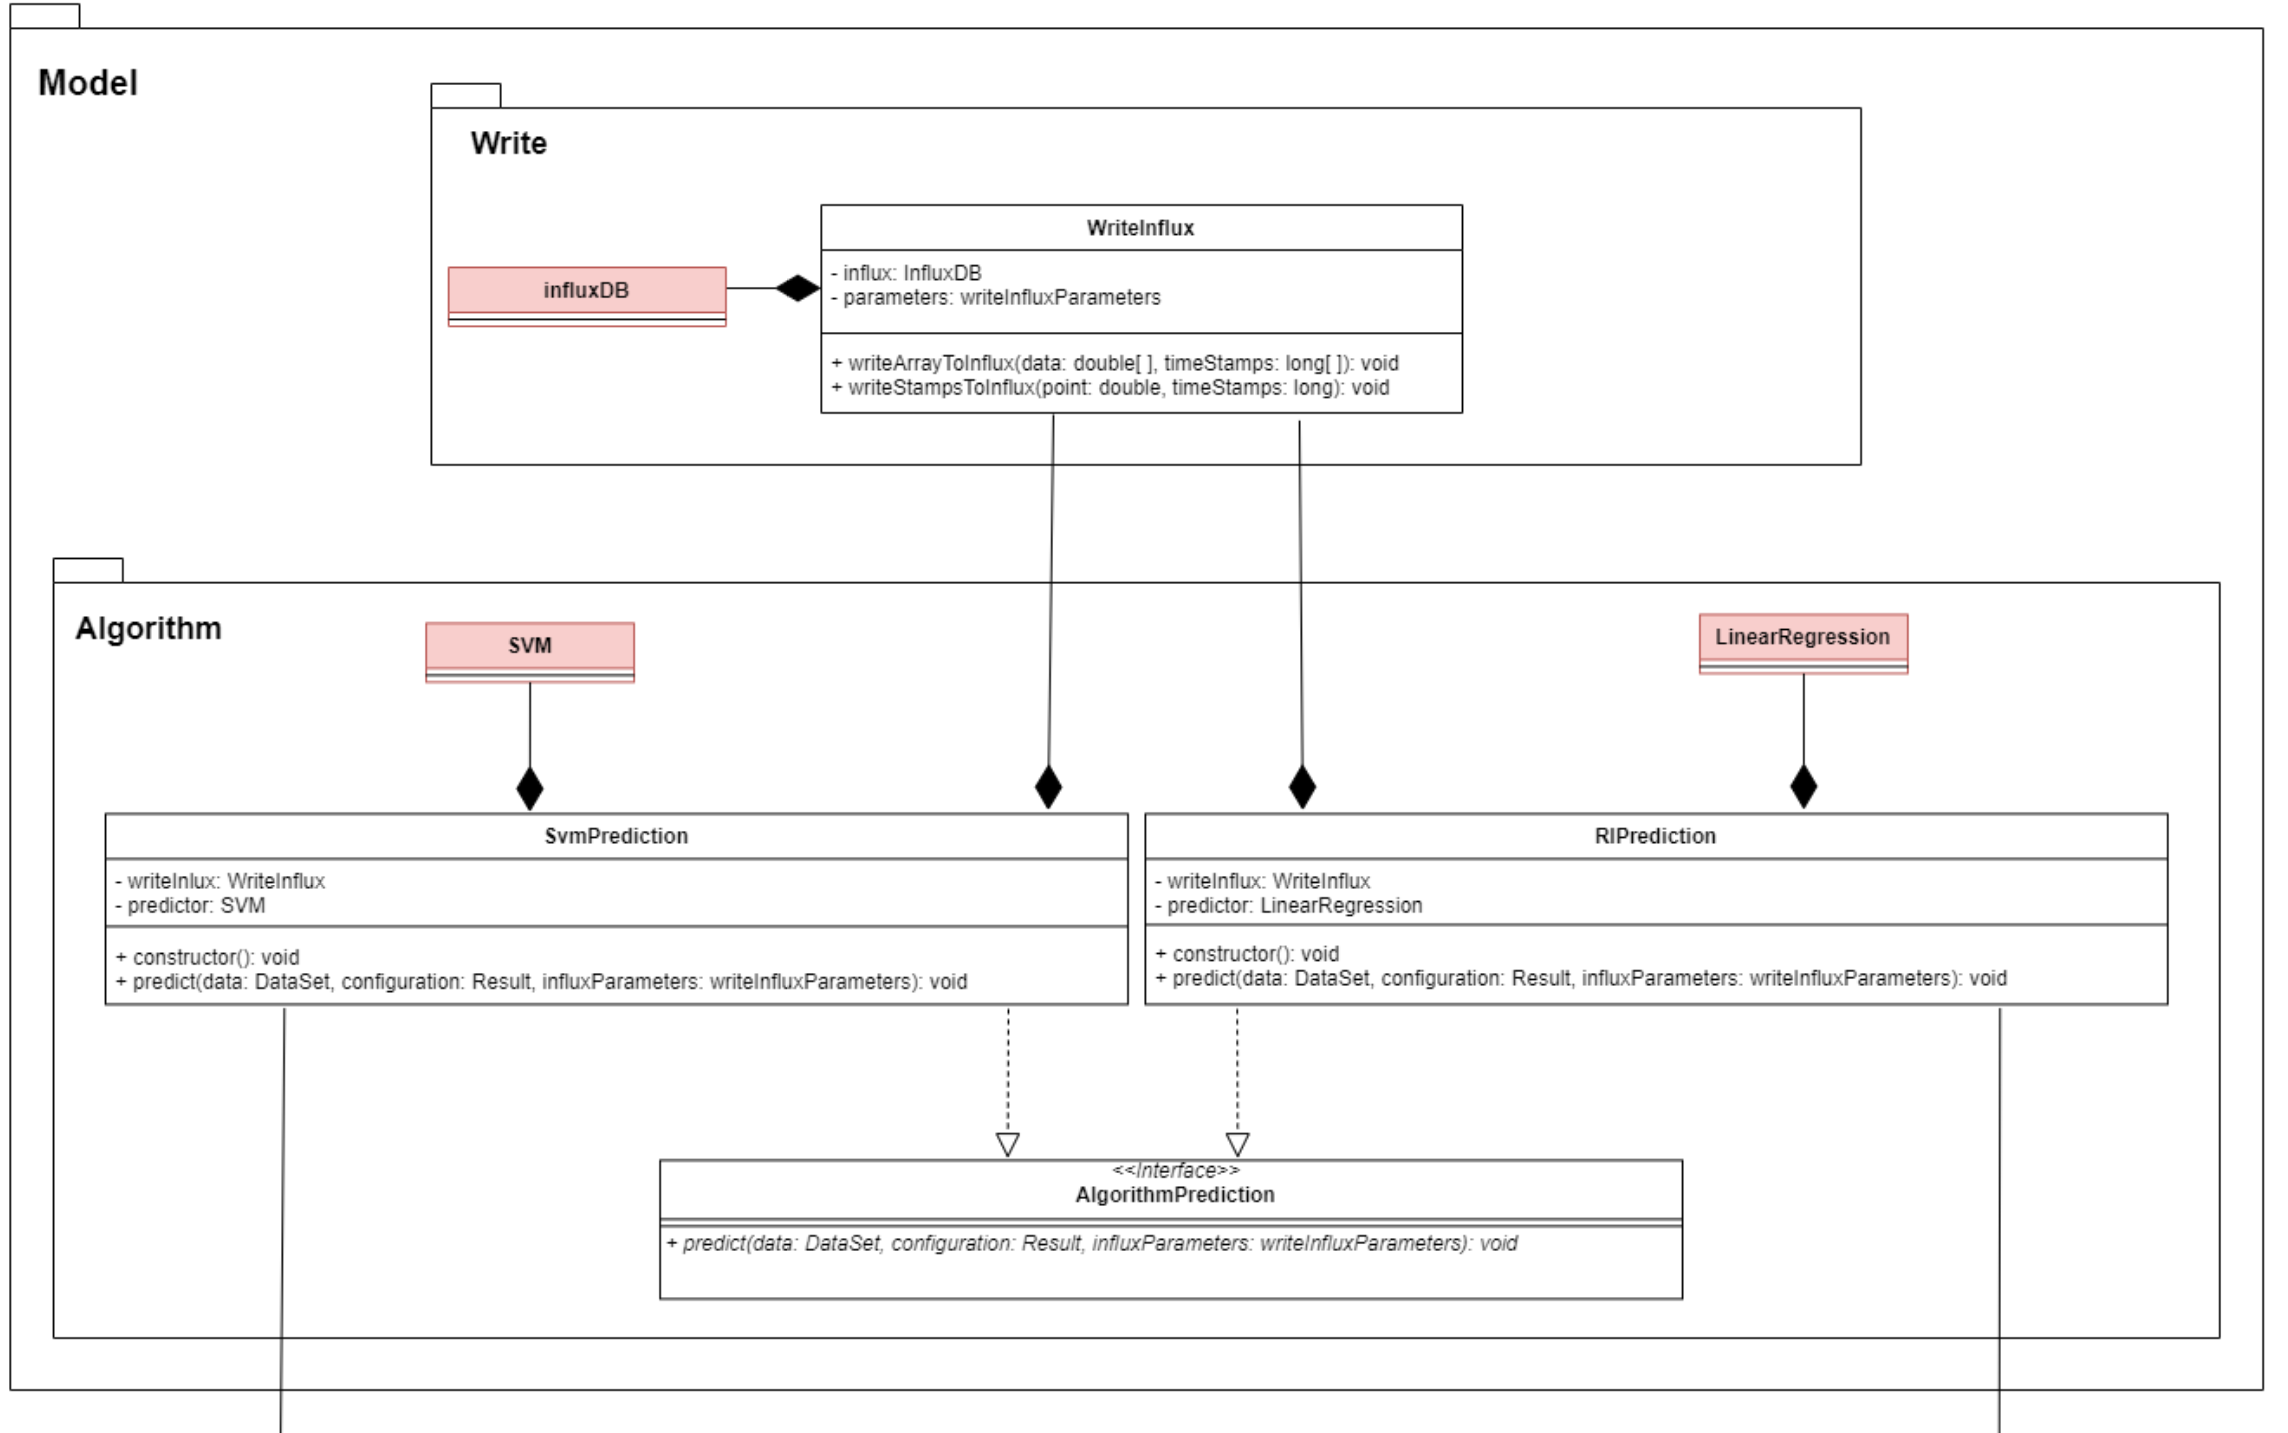
\includegraphics[width=\linewidth]{./img/Diagrammi/model-plug-in.png}
			\caption{Diagramma delle classi del Model}
		\end{figure}
	\end{figure}
\end{landscape}
\paragraph{View} \mbox{}
All'interno della View abbiamo inserito la componente Panel rappresentata dalla classe \textit{PanelCtrl} che estende \textit{MetricPanelControl} di Grafana\glo. Essa rappresenta il nostro pannello principale dal quale gli utenti possono interagire con il plug-in.
Ha una dipendenza di tipo composizione con un componente della libreria Plotly per la creazione dei grafici personalizzati e con la classe \textit{SelectinfluxDBCtrl} per la ricezione dei dati dalla datasource definita e connessa dall'utente. In questo modo, sfruttiamo il meccanismo di Grafana che dalla scrittura dei dati sul database a questo componente, permette l'aggiornamento continuo della View.
\mbox{}
\begin{landscape}
	\begin{figure}
		\begin{figure} [H]
			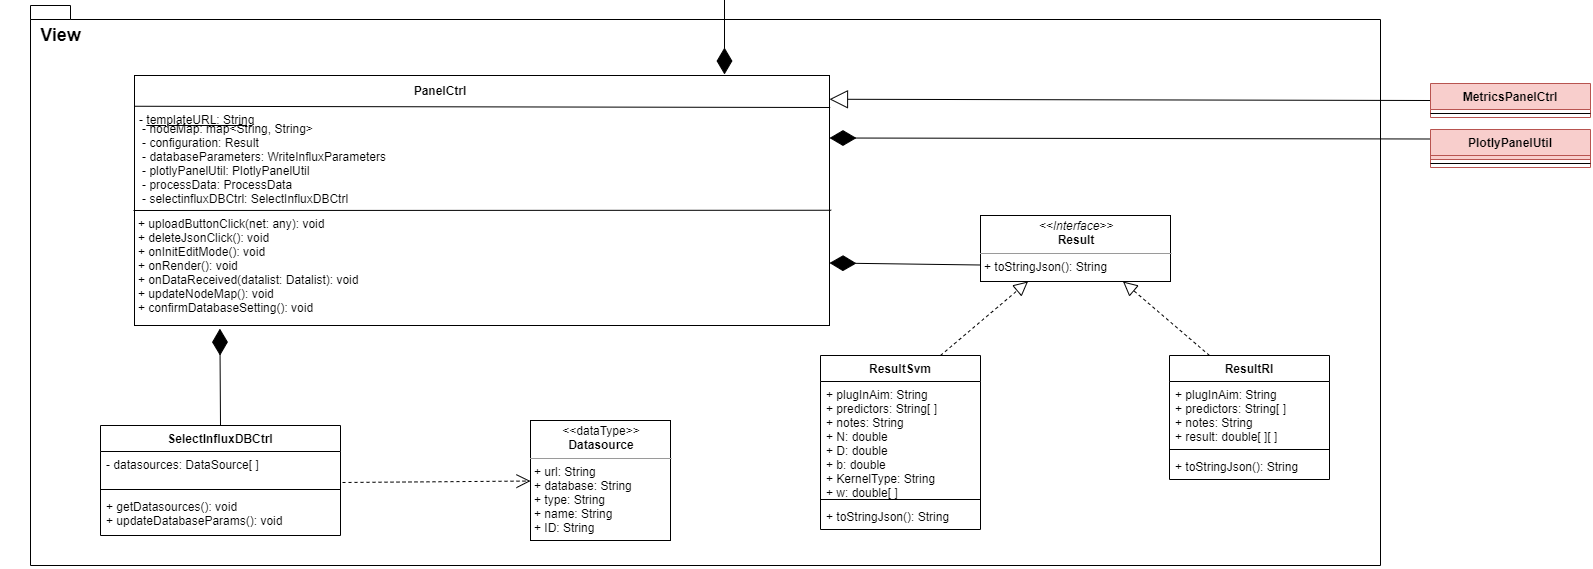
\includegraphics[width=\linewidth]{./img/Diagrammi/view-plug-in.png}
			\caption{Diagramma delle classi della View}
		\end{figure}
	\end{figure}
\end{landscape}
Infine, sempre all'interno di \textit{PanelCtrl}, c'è una dipendenza verso il componente \textit{ProcessData} del Controller che ne permette il collegamento.
\paragraph{Controller} \mbox{}
All'interno del Controller viene implementata la trasformazione dei dati ricevuti dalla View, che rappresentano le interazioni dell'utente con il nostro pannello, ad azioni da eseguire sul Model.
Abbiamo deciso di implementare un design pattern strategy ottenendo la seguente struttura:
\begin{itemize}
	\item \textbf{ProcessData}: è una classe concreta che rappresenta il context del nostro strategy. Al suo interno, infatti, viene scelto quale algoritmo di predizione processare sulla base dei dati e delle richieste ricevute. Inoltre essa ha una dipendenza di tipo aggregazione con l'interfaccia \textit{PerformPrediction};
	\item \textbf{PerformPrediction}: è un'interfaccia che rappresenta la strategia astratta. Essa definisce il contratto da rispettare per poter implementare una nuova classe concreta che processa i dati da fornire ad un determinato algoritmo;
	\item \textbf{ProcessSvm}: è una classe concreta che implementa \textit{PerformPrediction} e rappresenta il componente che processa e trasforma i dati da fornire per l'esecuzione dell'algoritmo Svm sul Model;
	\item \textbf{ProcessSvm}: è una classe concreta che implementa \textit{PerformPrediction} e rappresenta il componente che processa e trasforma i dati da fornire per l'esecuzione dell'algoritmo Rl sul Model;
\end{itemize}
\mbox{}
\begin{landscape}
	\begin{figure}
		\begin{figure} [H]
			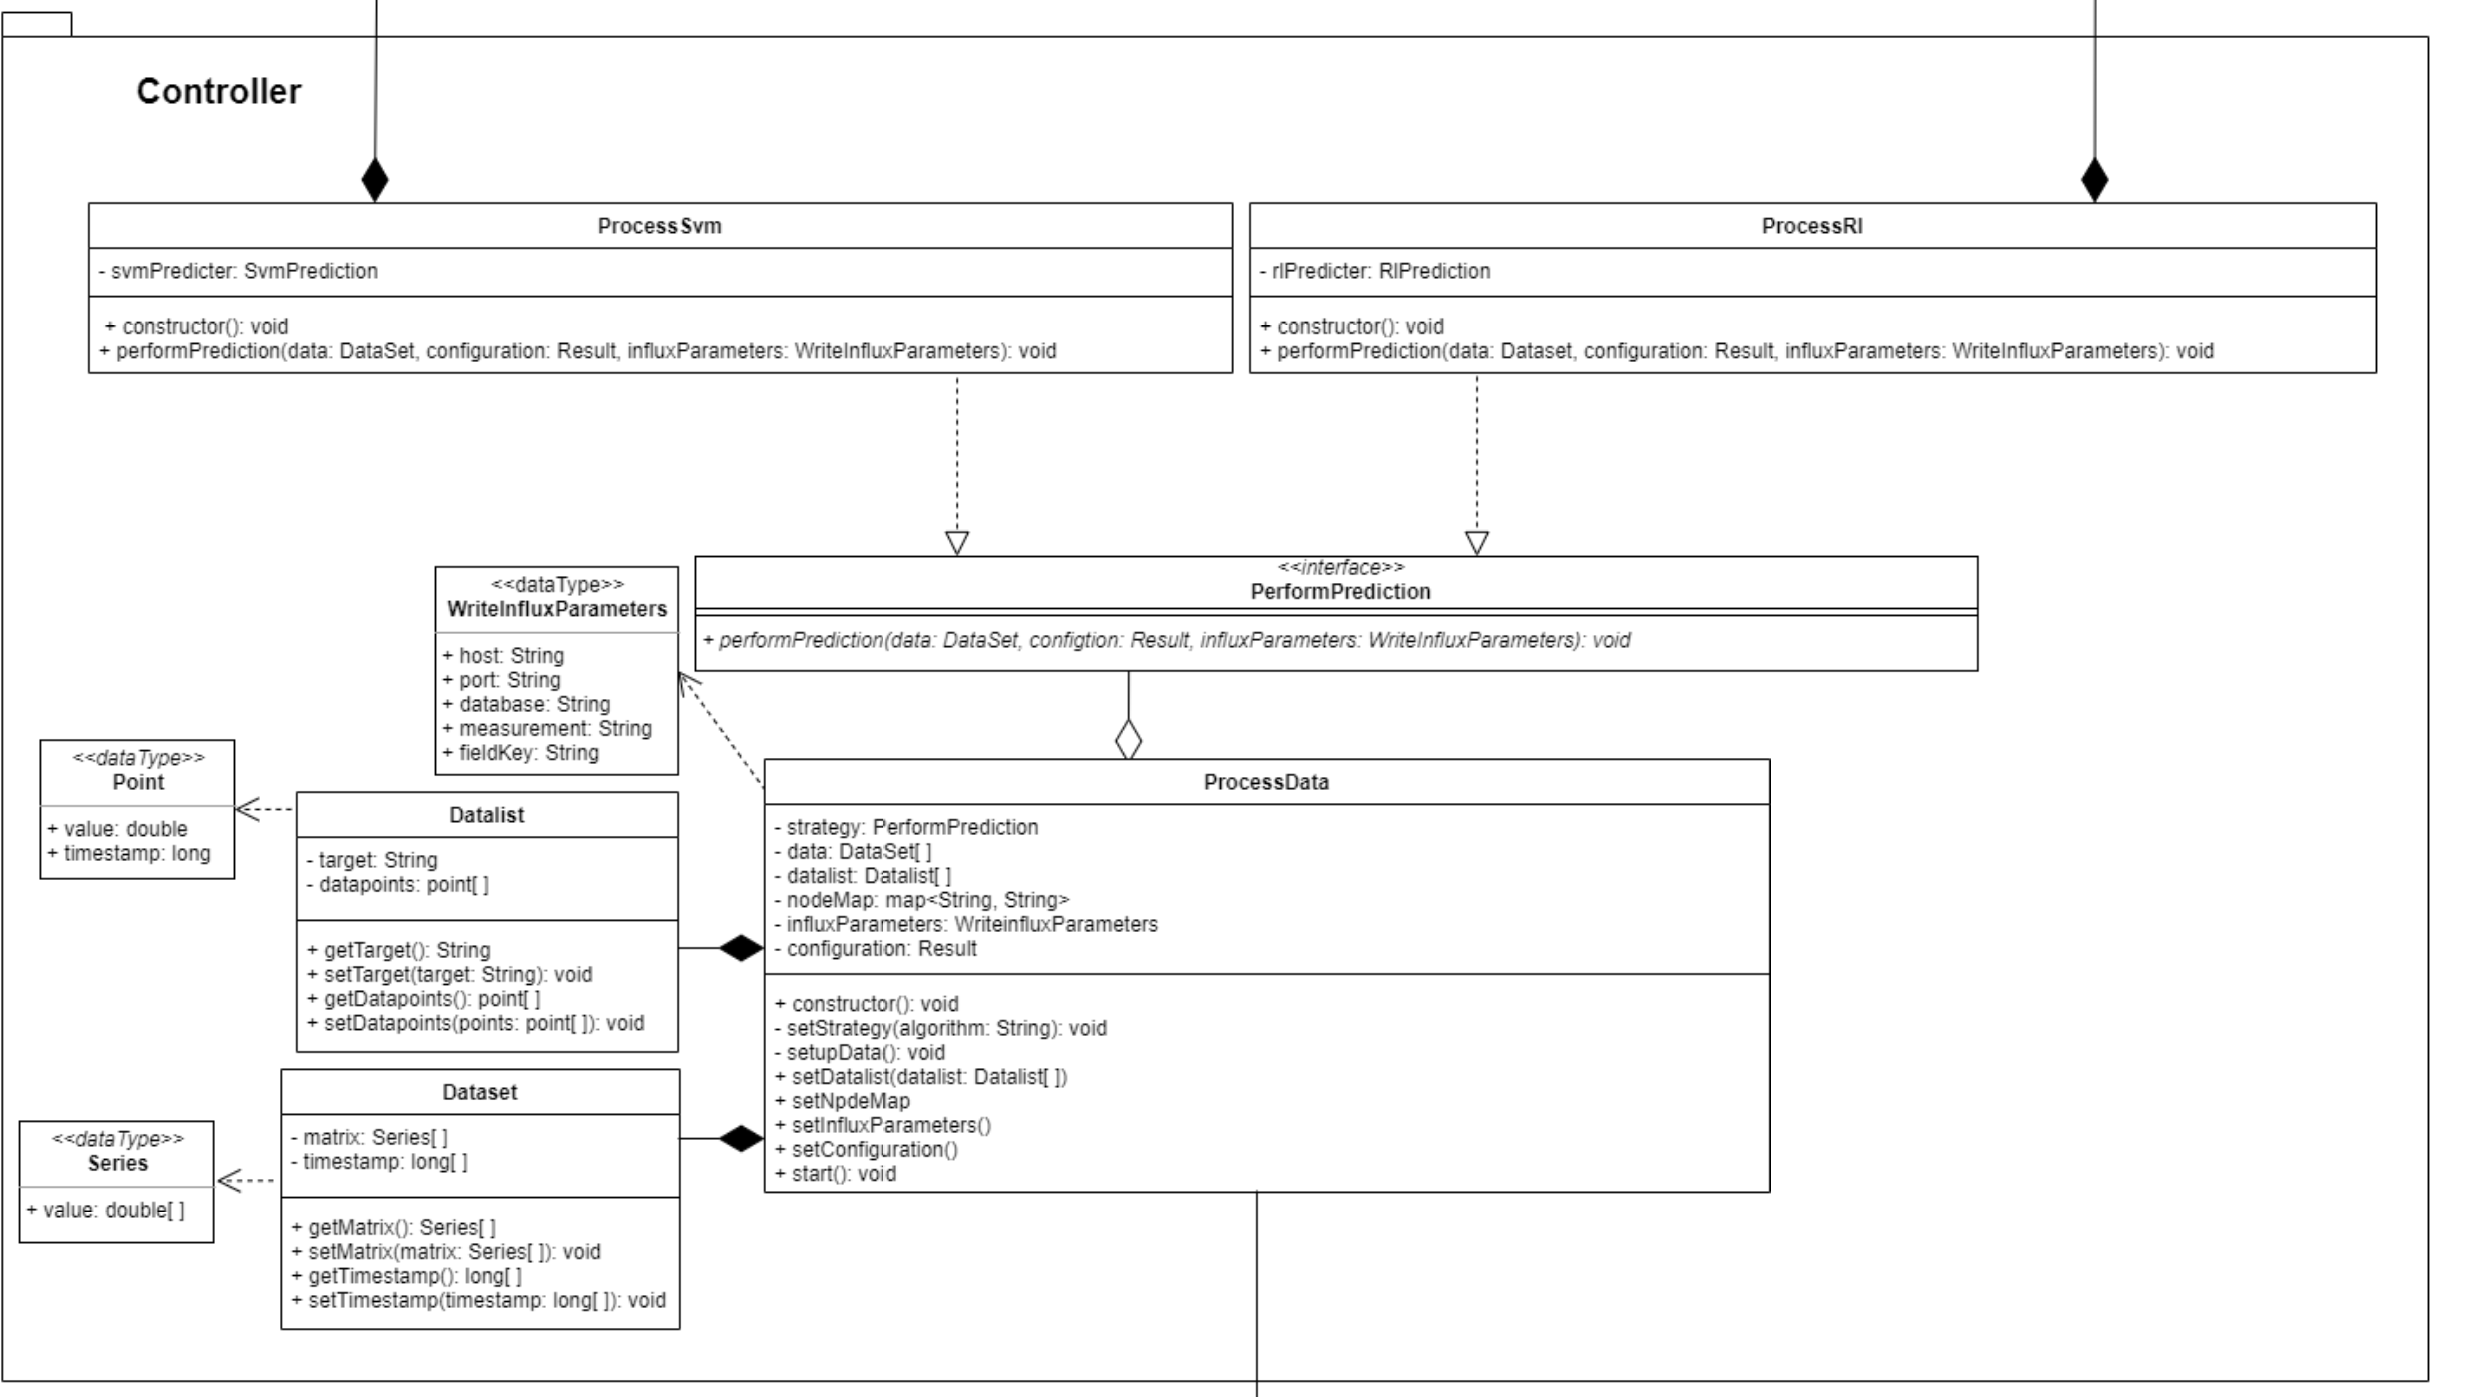
\includegraphics[width=\linewidth]{./img/Diagrammi/controller-plug-in.png}
			\caption{Diagramma delle classi del Controller}
		\end{figure}
	\end{figure}
\end{landscape}
Per spiegare meglio l'insieme di azioni compiute al fine di processare i dati per eseguire la predizione degli algoritmi, illustriamo un diagramma di sequenza che prende in esame SVM\glo. Il procedimento è indicativo anche per gli altri algoritmi.
\mbox{}
\begin{landscape}
	\begin{figure}
		\begin{figure} [H]
			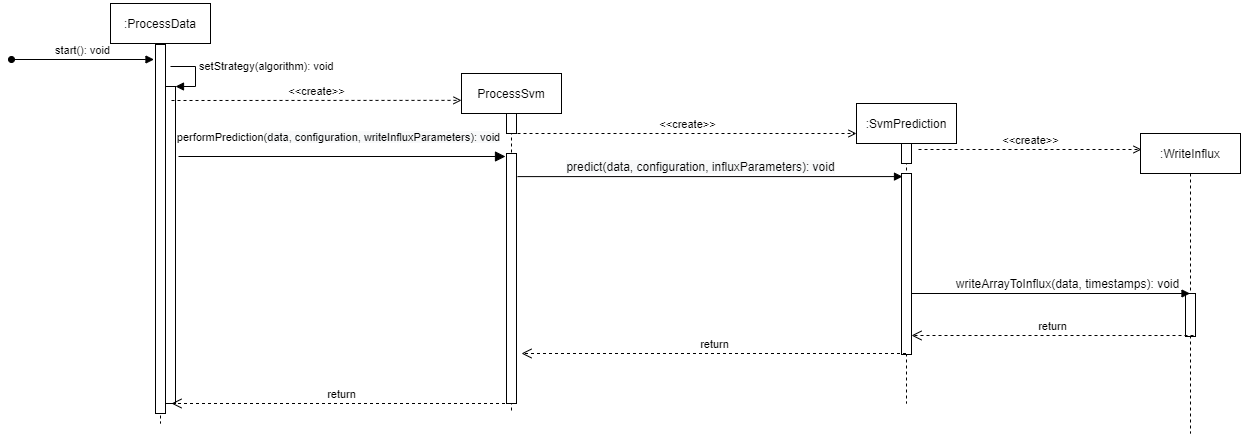
\includegraphics[width=\linewidth]{./img/Diagrammi/ds-plug-in.png}
			\caption{Diagramma di sequenza di processo dei dati per SVM}
		\end{figure}
	\end{figure}
\end{landscape}
	%ARCHITETTURA APP ESTERNA
\subsection{Applicazione esterna alla piattaforma Grafana}
Per poter visualizzare la suddivisione delle componenti dell'applicazione esterna e le dipendenze che sussistono tra loro ad alto livello, viene riportato il diagramma dei Package in allegato nel file \textit{diagramma-package-app.png}.
	\subsubsection{Progettazione architetturale}
	Abbiamo deciso di utilizzare un design pattern architetturale Model-View-ViewModel (MVVM) perché si adatta bene alle tecnologie che vengono utilizzate ovvero React ed Electron. In particolare, come si può vedere dalla figura seguente, la View invia dati a ViewModel che a sua volta fornisce delle risposte che permettono di tenere la vista sempre aggiornata. Questo scambio di dati è asincrono ed è fornito interamente da Electron. Inoltre abbiamo la comunicazione tra ViewModel e Model che avviene con la richiesta di esecuzione delle operazioni da parte del ViewModel ed la conseguente risposta da parte del Model. Anche questo scambio di messaggi è asincrono ed è implementato da un meccanismo di callback.
	\mbox{}
	\begin{landscape}
		\begin{figure}
			\begin{figure} [H]
				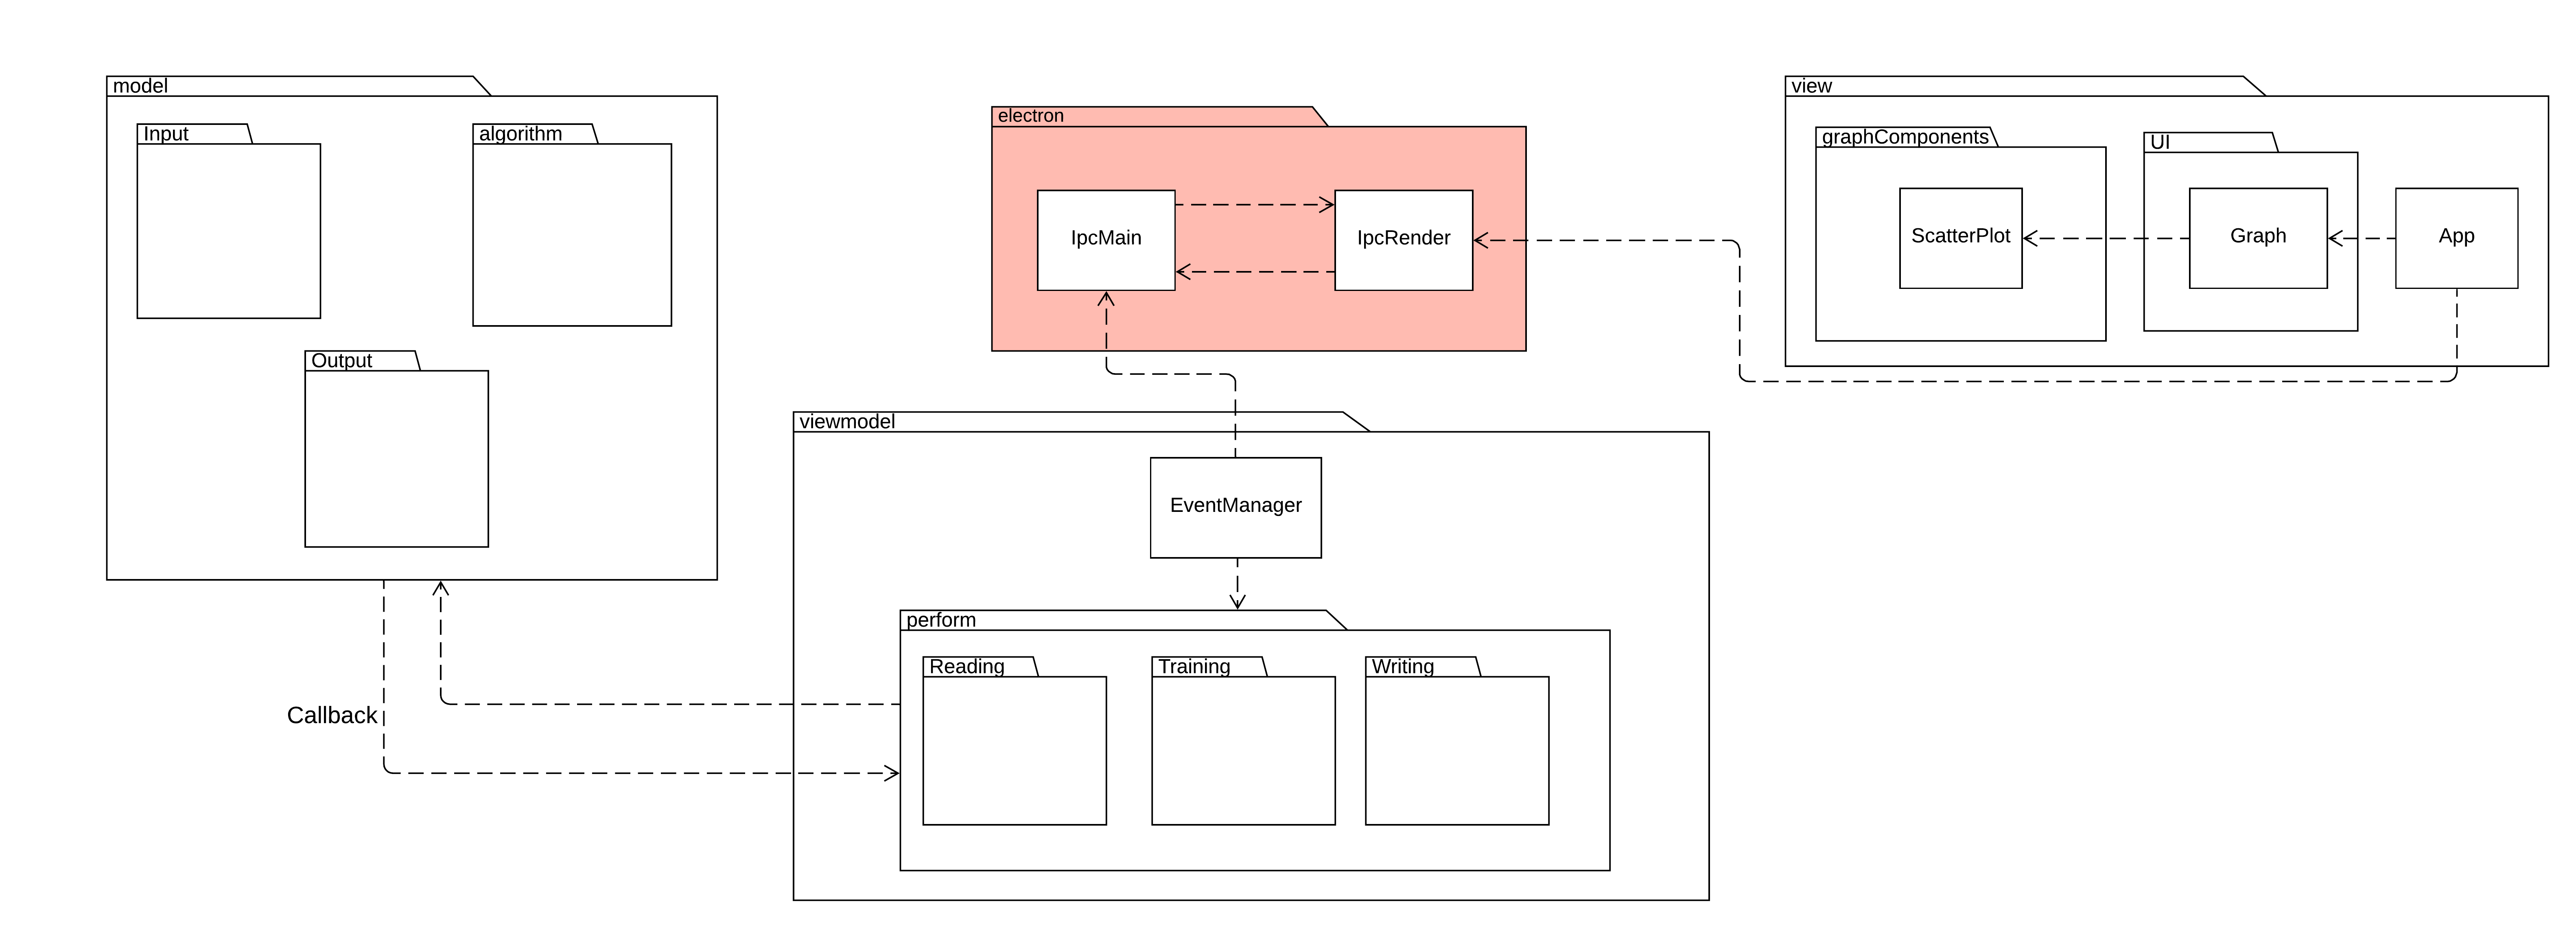
\includegraphics[width=\linewidth]{./img/Diagrammi/architettura-app.png}
				\caption{Diagramma dell'architettura dell'applicazione}
			\end{figure}
		\end{figure}
	\end{landscape}
	Analizzando i componenti, la nostra architettura è così strutturata: 
	\begin{itemize}
		\item \textbf{Model}: modulo che gestisce la business logic. Più in dettaglio esegue l'addestramento dei dati attraverso gli algoritmi di predizione e le operazioni di input/output dei file;
		\item \textbf{View}: modulo che gestisce la presentazione dei dati attraverso React;
		\item \textbf{ViewModel}: modulo che gestisce il binding tra View e Model con un meccanismo detto two-way-data-binding.
	\end{itemize}
	\subsubsection{Progettazione di dettaglio}
		Di seguito viene descritta in dettaglio la progettazione dell'applicazione. In allegato viene fornito il file \textit{diagramma-classi-app.png} contenente l'intero diagramma delle classi.
		\paragraph{Model} \mbox{} 
		\paragraph*{Algorithm} \mbox{} \\[1mm]
		Per la gestione degli algoritmi di addestramento abbiamo scelto di implementare due classi distinte \textit{SvmTrainer} e \textit{RlTrainer} che hanno una dipendenza di tipo composizione dalle rispettive classi delle librerie e del tipo di risultato ottenuto.
		All'interno di ognuna di esse viene fornita la possibilità di addestrare l'algoritmo e di calcolarne gli indici di qualità.
		\mbox{}
		\begin{landscape}
			\begin{figure}
				\begin{figure} [H]
					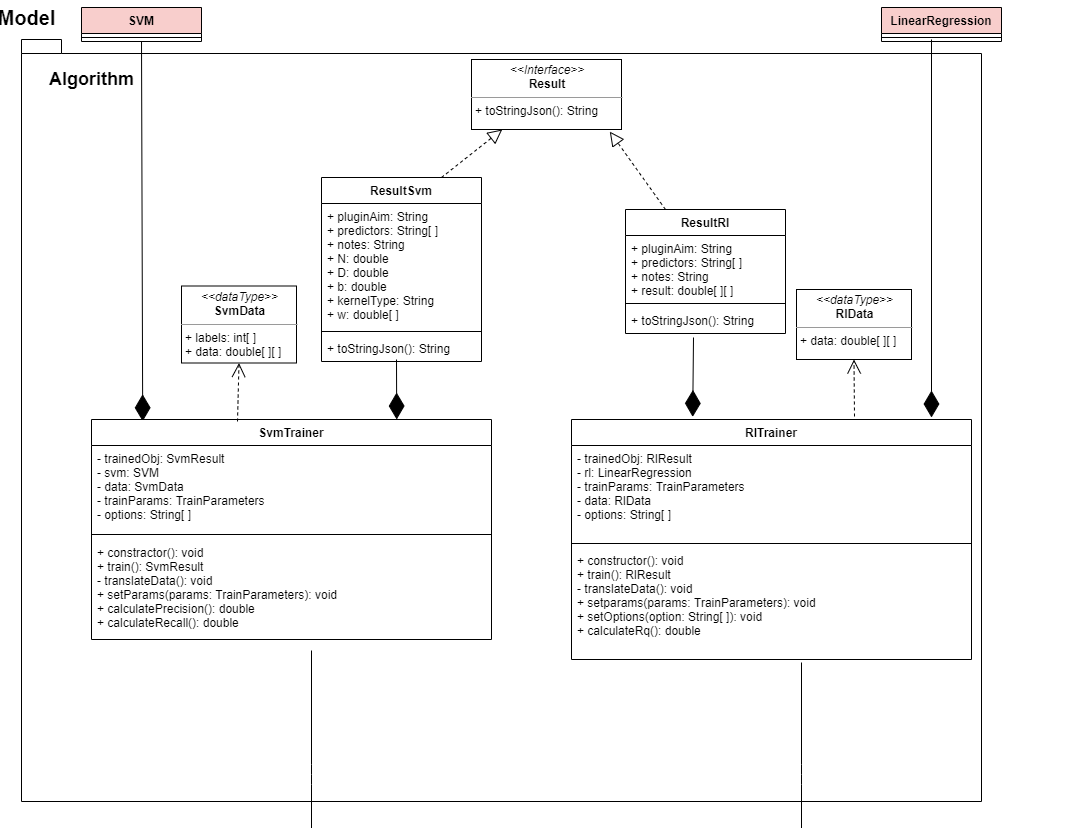
\includegraphics[width=\linewidth]{./img/Diagrammi/algorithm-app.png}
					\caption{Diagramma delle classi per gli algoritmi nel Model}
				\end{figure}
			\end{figure}
		\end{landscape}
		\paragraph*{Read} \mbox{} \\[1mm]
		Abbiamo riscontrato nella gestione dell'input che, indipendentemente dalla tipologia di file ricevuto, l'algoritmo per eseguire la lettura di quest'ultimo ha uno scheletro comune. È stato quindi deciso di implementare il design pattern template method.
		La classe astratta \textit{Read} implementa il metodo \textit{ReadFile(path, callback)} che rappresenta la parte comune dell'algoritmo di lettura da file. Inoltre contiene il metodo astratto \textit{parser(data, callback)} che invece rappresenta la trasformazione del contenuto del file sulla base della sua estensione e perciò viene implementato nelle classi concrete che estendono \textit{Read}. Nel nostro caso esse sono \textit{ReadCsv} e \textit{ReadJson}.
		\mbox{}
		%\begin{landscape}
			%\begin{figure}
				\begin{figure} [H]
					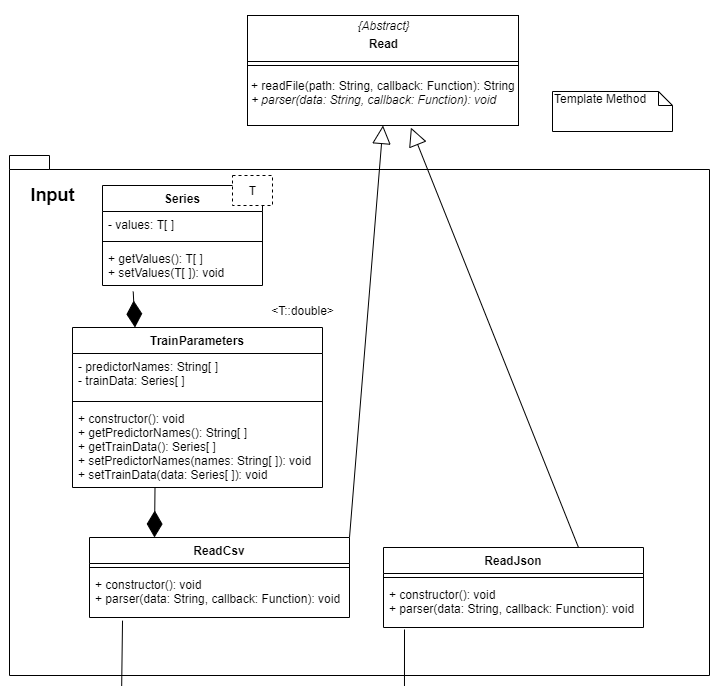
\includegraphics[width=\linewidth]{./img/Diagrammi/read-app.png}
					\caption{Diagramma delle classi per la Read nel Model}
				\end{figure}
			%\end{figure}
		%\end{landscape}
		\paragraph*{Write} \mbox{} \\[1mm]
		Anche nella gestione dell'output abbiamo riscontrato che, indipendentemente dalla tipologia di file su cui scrivere, l'algoritmo per eseguire la scrittura di quest'ultimo ha uno scheletro comune. È stato quindi deciso di implementare il design pattern template method.
		La classe astratta \textit{Write} implementa il metodo \textit{writeToDisk(path, name, data, notes, callback)} che rappresenta la parte comune dell'algortimo di scrittura su file. Inoltre contiene il metodo astratto \textit{parser(data, callback)} che invece rappresenta la trasformazione dell'oggetto che vogliamo scrivere sul file nel formato corretto. Nel nostro caso abbiamo implementato la classe concreta \textit{WriteJson} ma è estendile a tutti i formati di file desiderati estendendo \textit{Write}.
		\mbox{}
		%\begin{landscape}
		%	\begin{figure}
				\begin{figure} [H]
					\begin{center}
						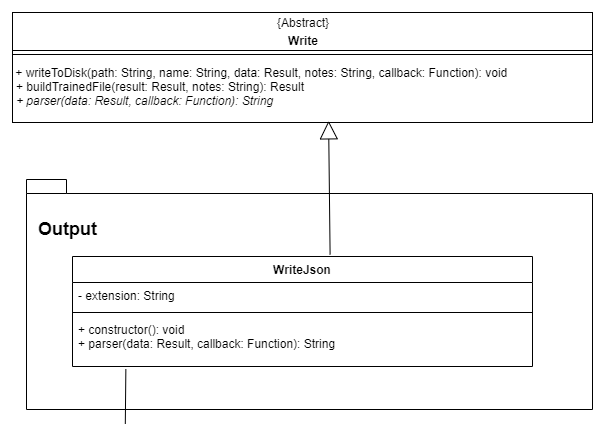
\includegraphics[width=120mm]{./img/Diagrammi/write-app.png}
					\end{center}
					\caption{Diagramma delle classi per la Write nel Model}
				\end{figure}
		%	\end{figure}
		%\end{landscape}

		\paragraph{View} \mbox{} \\[1mm]
		La View è realizzata attraverso dei componenti di React contenuti nella classe principale \textit{App} attraverso una dipendenza di tipo composizione. Grazie all'estensione della classe \textit{Component} di React, otteniamo il metodo \textit{render()} che renderizza i componenti visualizzandoli nell'interfaccia utente.
		Infine per l'implementazione del grafico di addestramento, utilizziamo la libreria D3.
		\mbox{}
		%\begin{landscape}
		%	\begin{figure}
				\begin{figure} [H]
					\begin{center}
						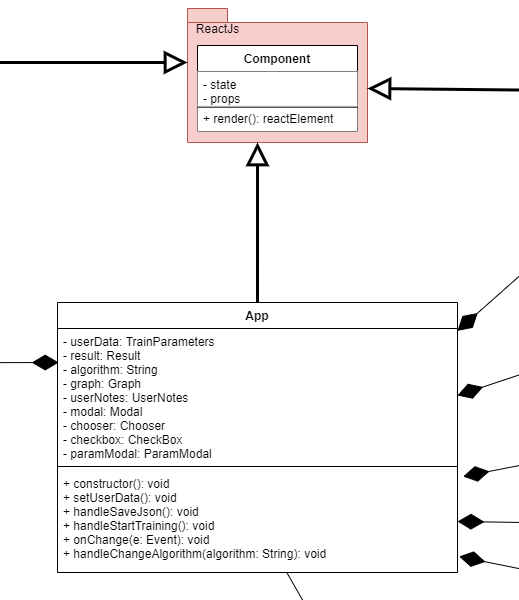
\includegraphics[width=100mm]{./img/Diagrammi/view-app.png}
					\end{center}
					\caption{Diagramma delle classi della View}
				\end{figure}
		%	\end{figure}
		%\end{landscape}
	
		\paragraph{ViewModel} \mbox{} \\[1mm]
		La ViewModel contiene i dati da visualizzare nella vista e le trasformazioni per richiamare le operazioni da eseguire nel modello.
		In particolare è legato alla View tramite Electron che gestisce la loro comunicazione in modo asincrono appoggiandosi al nostro componente \textit{EventManager} e al Model attraverso il meccanismo asincrono di callback.
		Abbiamo riscontrato la necessità di implementare il design pattern strategy in tre casi diversi:
		\paragraph*{Algorithm} \mbox{}
		\begin{itemize}
			\item \textbf{ProcessTraining}: è una classe concreta che rappresenta il context. In essa viene scelto quale algoritmo addestrare sulla base dei dati ricevuti ed ha una dipendenza di tipo aggregazione dall'interfaccia \textit{PerformTraining};
			\item \textbf{PerformTraining}: è un'interfaccia che rappresenta la strategia astratta. Essa definisce il contratto da rispettare per le classi che implementano il process degli algoritmi di addestramento;
			\item \textbf{PerformTrainingSvm}: è una classe concreta che implementa \textit{PerformTraining} e rappresenta il componente che esegue la trasformazione ed il controllo dei dati per richiamare correttamente l'algortimo di addestramento SVM\glosp nel Model.
			\item \textbf{PerformTrainingRl}: è una classe concreta che implementa \textit{PerformTraining} e rappresenta il componente che esegue la trasformazione ed il controllo dei dati per richiamare correttamente l'algortimo di addestramento RL\glosp nel Model.
		\end{itemize}
		\mbox{}
		\begin{landscape}
			\begin{figure}
				\begin{figure} [H]
					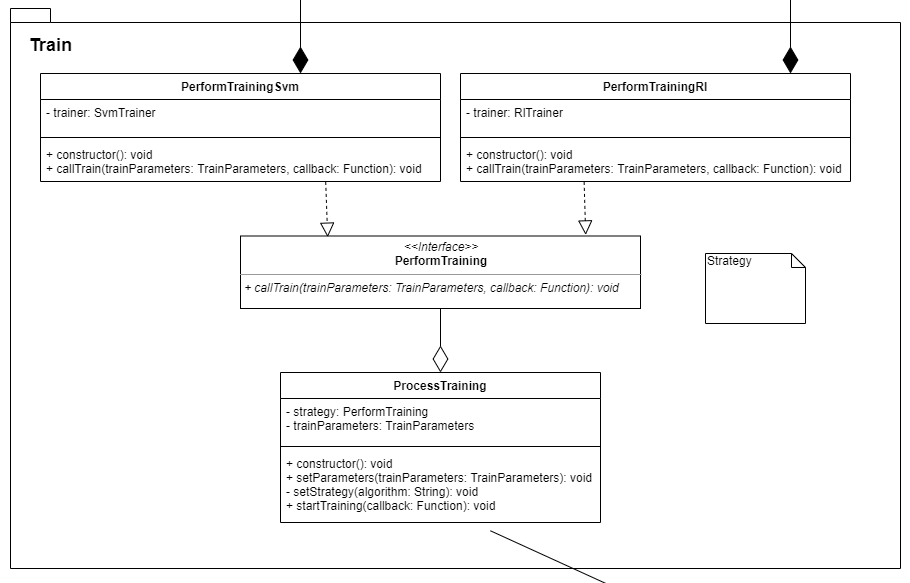
\includegraphics[width=\linewidth]{./img/Diagrammi/ViewModel-train-app.png}
					\caption{Diagramma delle classi per il training nel ViewModel}
				\end{figure}
			\end{figure}
		\end{landscape}
		Per spiegare meglio l'insieme di azioni compiute al fine di processare i dati per eseguire l'addestramento degli algoritmi, illustriamo un diagramma di sequenza che prende in esame SVM\glo. Per gli altri algoritmi il procedimento è simile.
		\mbox{}
		\begin{landscape}
			\begin{figure}
				\begin{figure} [H]
					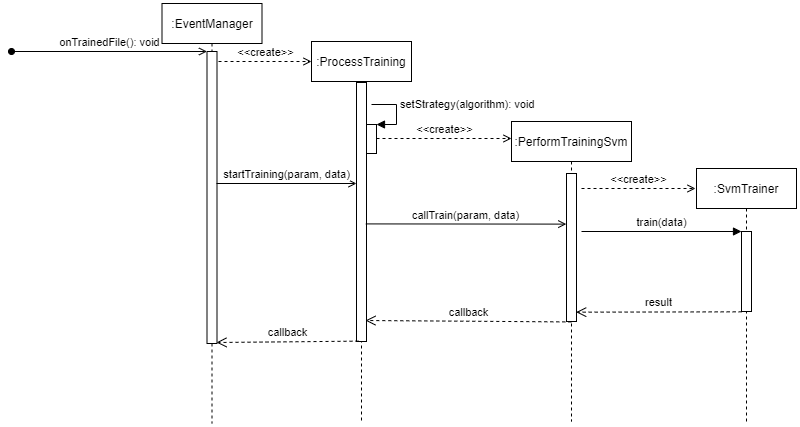
\includegraphics[width=\linewidth]{./img/Diagrammi/ds-app.png}
					\caption{Diagramma di sequenza di processo dei dati per SVM}
				\end{figure}
			\end{figure}
		\end{landscape}
		\paragraph*{Read} \mbox{}
		\begin{itemize}
			\item \textbf{ProcessReading}: è una classe concreta che rappresenta il context. In essa viene scelta la tipologia di file da leggere sulla base dei dati ricevuti ed ha una dipendenza di tipo aggregazione dall'interfaccia \textit{PerformReading};
			\item \textbf{PerformReading}: è un'interfaccia che rappresenta la strategia astratta. Essa definisce il contratto da rispettare per le classi che implementano la lettura da file;
			\item \textbf{PerformReadingCsv}: è una classe concreta che implementa \textit{PerformReading} e rappresenta il componente che esegue le trasformazioni necessarie per richiamare la correttamente l'algoritmo di lettura di un file Csv del Model;
			\item \textbf{PerformReadingJSon}: è una classe concreta che implementa \textit{PerformReading} e rappresenta il componente ch esegue le trasformazioni necessarie per richiamare la correttamente l'algoritmo di lettura di un file Json del Model.
		\end{itemize}
		\mbox{}
		%\begin{landscape}
		%	\begin{figure}
				\begin{figure} [H]
					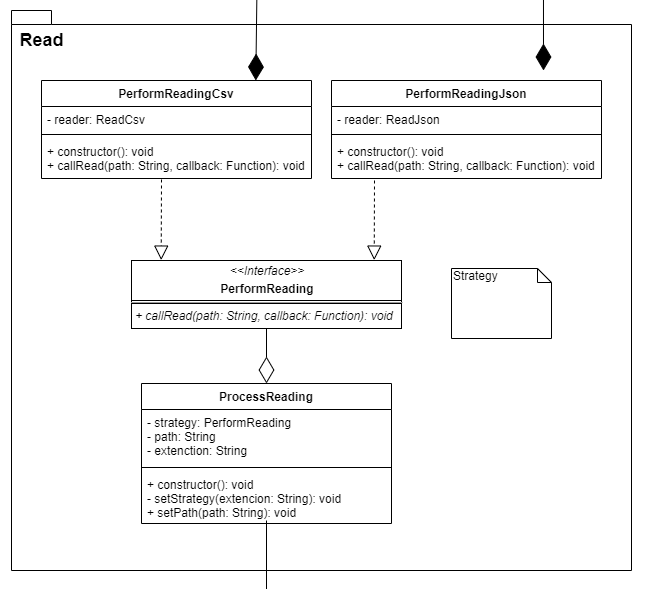
\includegraphics[width=\linewidth]{./img/Diagrammi/ViewModel-read-app.png}
					\caption{Diagramma delle classi per la Read nel ViewModel}
				\end{figure}
		%	\end{figure}
		%\end{landscape}
		\paragraph*{Writing} \mbox{} \\[1mm]
		\begin{itemize}
			\item \textbf{ProcessWriting}: è una classe concreta che rappresenta il context. in essa viene scelta la tipologia di file su cui scrivere in base ai dati ricevuti ed ha una dipendenza di tipo aggregazione dall'interfaccia \textit{PerformWriting};
			\item \textbf{PerformWriting}: è un'interfaccia che rappresenta la strategia astratta. Essa definisce il contratto da rispettare per le classi che implementano la lettura da file;
			\item \textbf{PerformWritingJson}: è una classe concreta che implementa \textit{PerformWriting} e rappresenta il componente che esegue le trasformazioni necessarie per richiamare correttamente l'algoritmo di scrittura di un file Json del Model.
		\end{itemize}
		\mbox{}
		%\begin{landscape}
		%	\begin{figure}
				\begin{figure} [H]
					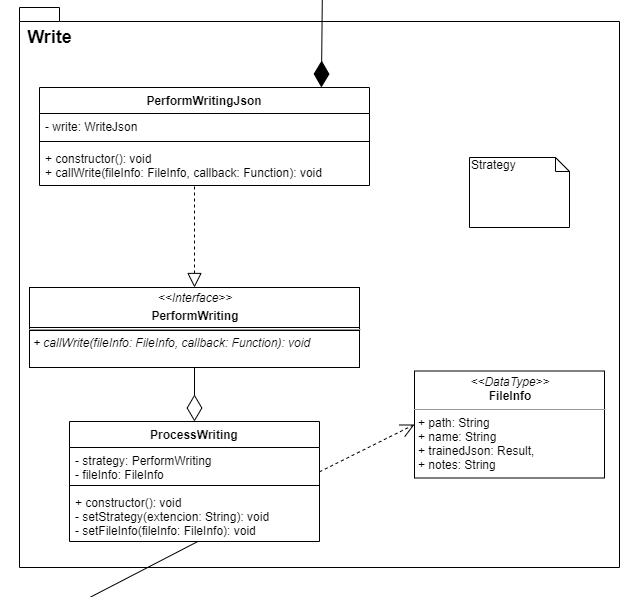
\includegraphics[width=\linewidth]{./img/Diagrammi/ViewModel-write-app.png}
					\caption{Diagramma delle classi per la Write nel ViewModel}
				\end{figure}
		%	\end{figure}
		%\end{landscape}
		
	\pagebreak
	\section{Estensibilità del prodotto}
	\subsection{Supporto a nuovi algoritmi di predizione}
	Al momento sono stati implementati gli algoritmi di addestramento e di predizione di Support Vector Machine lineare e di Regressione lineare. Grazie alla struttura dell'architettura è possibile aggiungere le varianti delle famiglie di algoritmi di Support Vector Machine e di Regressione quali non lineari, esponenziali e logaritmiche.
	Per realizzare ciò, è sufficiente eseguire il seguente procedimento per ogni nuovo algoritmo. Creare una nuova implementazione dell'interfaccia \textit{PerformTraining} con la relativa classe nel Model all'interno dell'applicazione ed una nuova implementazione delle interfacce \textit{PerformPrediction} e \textit{AlgorithmTrainer} nel plug-in.
	\subsection{Supporto a nuove tipologie di file}
		\subsubsection{Lettura}
		Viene offerta la possibilità di ampliare le tipologia di file che vengono utilizzate per la lettura dei dati ricevuti in input di addestramento nell'applicazione. Questo è possibile grazie all'implementazione del template method. Infatti è sufficiente estendere la classe astratta \textit{Read} e successivamente implementare il metodo \textit{parser()} per eseguire il parse dei dati nel formato desiderato.
		\subsubsection{Scrittura}
		Viene offerta la possibilità di ampliare le tipologia di file che vengono utilizzate per la scrittura dei dati risultanti dall'addestramento nell'applicazione. Questo è possibile grazie all'implementazione del template method. Infatti è sufficiente estendere la classe astratta \textit{Write} e successivamente implementare il metodo \textit{parser()} per eseguire il parse dei dati nel formato desiderato.
	\pagebreak
	\section{Struttura dei file}
	\subsection{Struttura del Json}
	I file Json che contengono la configurazione degli algoritmi di addestramento devono essere strutturati nei modi qui sotto indicati.
		\subsubsection{Regressione Lineare}
		\begin{itemize}
			\item \textbf{author} indica l'autore del file
			\item \textbf{version} indica la versione dell'applicazione con cui si è creato il file
			\item \textbf{date} indica la data in cui è stato creato il file
			\item \textbf{time} indica l'ora in cui è stato creato il file
			\item \textbf{pluginAim} indica l'algoritmo addestrato, in questo caso deve essere "rl"
			\item \textbf{predictors} elenco delle etichette dei predittori
			\item \textbf{result} elenco dei coefficienti risultati dall'addestramento
			\item \textbf{notes} eventuali note inserite durante l'addestramento
		\end{itemize}
		\mbox{}
		\begin{figure} [H]
			\begin{center}
				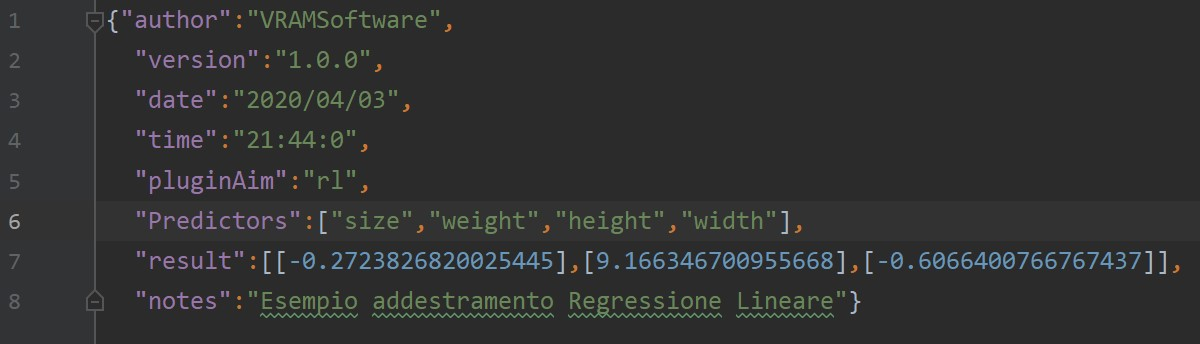
\includegraphics[width=\linewidth]{./img/jsonRl.jpg}
			\end{center}
			\caption{Esempio file Json per la Regressione Lineare}
		\end{figure}
		\mbox{}
		\subsubsection{Support Vector Machine}
			\begin{itemize}
				\item \textbf{author} indica l'autore del file
				\item \textbf{version} indica la versione dell'applicazione con cui si è creato il file
				\item \textbf{date} indica la data in cui è stato creato il file
				\item \textbf{time} indica l'ora in cui è stato creato il file
				\item \textbf{pluginAim} indica l'algoritmo addestrato, in questo caso deve essere "svm"
				\item \textbf{predictors} elenco delle etichette dei predittori
				\item \textbf{trainData} elenco dei dati addestrati
				\item \textbf{trainLabels} elenco delle label dei dati addestrati
				\item \textbf{result} elenco dei parametri risultati dall'addestramento, in particolare 
				\begin{itemize}
					\item \textbf{N} indica il numero di dati addestrati
					\item \textbf{D} indica la dimensione dei dati addestrati
					\item \textbf{b} indica lo scalare risultato dall'addestramento
					\item \textbf{kernelType} indica il tipo di kernel utilizzato, attualmente è implementato solo il kernel "linear"
					\item \textbf{w} indica il vettore risultato dall'addestramento					
				\end{itemize}
				\item \textbf{notes} eventuali note inserite durante l'addestramento
			\end{itemize}
		\mbox{}
		\begin{figure} [H]
			\begin{center}
				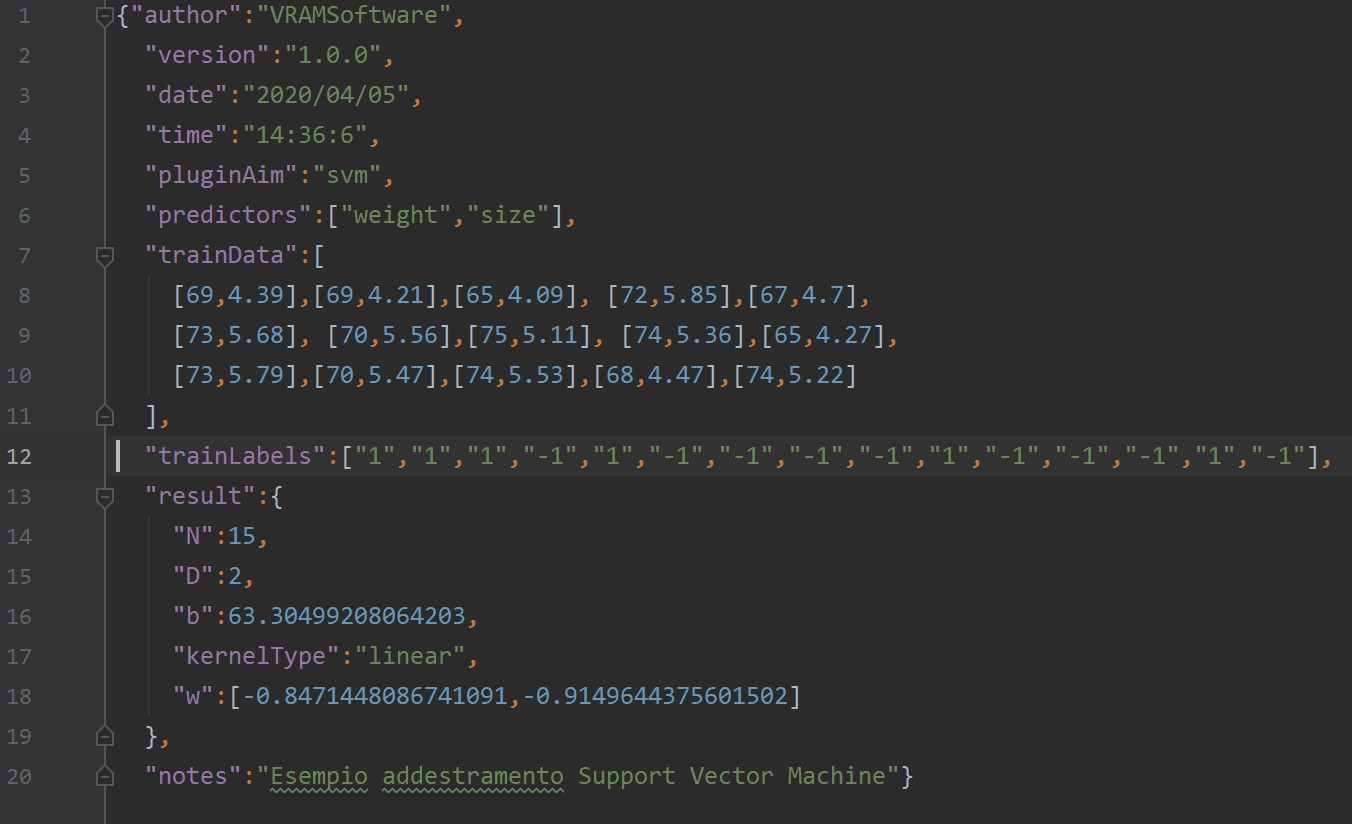
\includegraphics[width=\linewidth]{./img/jsonSvm.jpg}
			\end{center}
			\caption{Esempio file Json per la Support Vector Machine}
		\end{figure}
		\mbox{} \\ \\ 
		Se si desiderano ulteriori informazioni sulle regole sintattiche dei file JSON, si consiglia di consultare la documentazione W3C disponibile al seguente link:
		\\[0.2cm]
		\hspace*{10mm}
		\url{https://www.w3schools.com/js/js_json_syntax.asp}
		
	\subsection{Struttura del CSV}
	La struttura del file .csv è indipendente dall'algoritmo che si vuole addestrare.
	Deve presentare i valori di ogni predittore divisi per colonne, la prima riga di ogni colonna deve indicare l'etichetta associata al predittore. \\
	A seconda del caso devono essere presenti una o più colonne per i predetti, la prima riga di ogni colonna deve indicare l'etichetta associata al predetto.
	\mbox{}
	\begin{figure} [H]
		\begin{center}
			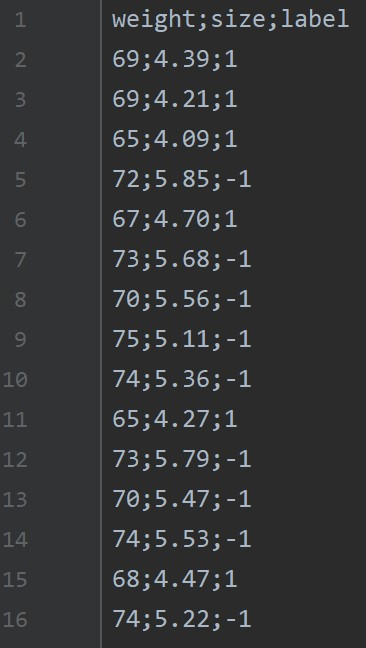
\includegraphics[width=50mm]{./img/csv1.jpg}
		\end{center}
		\caption{Esempio file csv}
	\end{figure}
	\mbox{}
	I file .csv possono eventualmente essere gestiti tramite fogli di calcolo
	\mbox{}
	\begin{figure} [H]
		\begin{center}
			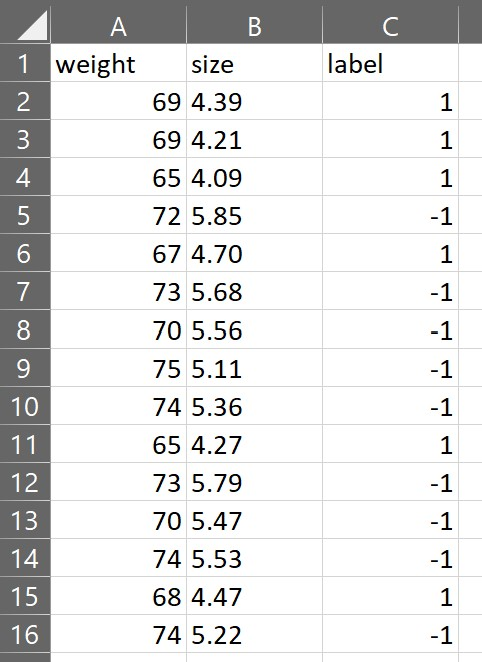
\includegraphics[width=50mm]{./img/csv2.jpg}
		\end{center}
		\caption{Esempio file csv su Microsoft Excel}
	\end{figure}
	\mbox{} 
	% ...
	%\input{res/inserire nome sezione n} 
	
	\appendix
	\section{Glossario}

%\subsection*{C}
%\subsubsection*{CSV}
%Il comma-separated values (abbreviato in CSV) è un formato di file basato su file di testo utilizzato per l'importazione ed esportazione di una tabella di dati. 

\subsection*{D}
\subsubsection*{Datasource}
Una datasource è una sorgente di dati in Grafana. Solitamente si tratta di un database.

\subsubsection*{Dashboard}
In italiano cruscotto; interfaccia che permette all'utente di tenere sotto controllo gli indicatori più importanti dell'ambiente in cui sta lavorando. È caratteristica fondamentale l'aggiornamento automatico dei dati, senza che vi debba essere un'interazione con l'utente.

\subsection*{G}
\subsubsection*{Grafana}
Software ad uso generico per la produzione di cruscotti informativi (dashboard in inglese) e composizione di grafici. Viene utilizzato come un'applicazione web.

\subsection*{I}
\subsubsection*{InfluxDB}
InfluxDB è un database basato sul concetto di serie temporale. InfluxDB è specializzato e
ottimizzato per il salvataggio e la lettura di serie temporali: record salvati in ordine temporale
e caratterizzati dal timestamp, ovvero un campo che indica una data. InfluxDB è utilizzato
per lo più in ambiti in cui è necessario salvare valori generati da sensori oppure analytics in
tempo reale.

%\subsection*{J}
%\subsubsection*{JSON}
%Acronimo di JavaScript Object Notation, è un formato adatto all'interscambio di dati fra applicazioni client/server. È basato sul linguaggio JavaScript Standard ma ne è indipendente.

\subsection*{M}
\subsubsection*{Machine learning}
Il machine learning (in italiano apprendimento automatico) è una branca dell'intelligenza artificiale che utilizza metodi statistici per migliorare progressivamente la performance di un algoritmo nell'identificare pattern nei dati.

\subsection*{P}
\subsubsection*{Predittore}
Dati o variabili su cui applico le tecniche di regressione o di classificazione per ottenere un dato la cui diretta rilevazione sarebbe impossibile o troppo onerosa.

\subsubsection*{Prodotto}
Si definisce prodotto qualsiasi bene scambiabile sul mercato che può rispondere alle esigenze di un compratore. Un esempio di prodotto informatico è il software che è composto dal codice e dalla documentazione.	

\subsubsection*{RL}
Acronimo di Regressione lineare, algoritmo di machine learning\glosp che ha la funzione di prevedere un valore di una variabile dipendente (y) in base a una determinata variabile indipendente (x) secondo una relazione di tipo lineare.
\subsection*{S}
\subsubsection*{SVM}
Acronimo di Support Vector Machine; algoritmo di apprendimento automatico supervisionato che può essere utilizzato sia per scopi di classificazione che di regressione.


\end{document}